%================================================
\chapter{コホモロジー環・ポアンカレ双対・交叉形式}\label{ch:06}
% 18問
%================================================

\section{物理からの動機}

\subsection*{位相項は「流束の積」である}
4次元のゲージ理論には、計量によらない\term{位相項}{topological term}
\[
S_\theta=\theta\,k,\qquad k=\frac{1}{8\pi^2}\int_X\tr F\wedge F
\]
を加えることができる（記法と規約の $k$）。$\R^4$ 上の $SU(N)$ インスタントンでは $k\in\Z$ なので $e^{iS_\theta}$ は $\theta\to\theta+2\pi$ で不変であり、$\theta$ は角度変数である。ところが $U(1)$ ゲージ理論をコンパクトな4次元多様体 $X$ 上で考えると、$F/2\pi$ はそれ自体が整数係数のコホモロジー類 $c\in H^2(X;\Z)$ を代表し（第5章のディラック量子化）、
\[
k=\frac{1}{8\pi^2}\int_X F\wedge F=\frac12\int_X\frac{F}{2\pi}\wedge\frac{F}{2\pi}=\frac12\,Q(c,c)
\]
となる。ここで $Q(c,c)$ は「2次のコホモロジー類どうしの積を $X$ 上で積分した整数」で、$X$ の\textbf{交叉形式}と呼ばれる（本章）。$Q(c,c)$ が常に偶数なら $k\in\Z$ で $\theta$ の周期は $2\pi$、奇数になりうるなら $k\in\tfrac12\Z$ で周期は $4\pi$ になる（問題 \ref{ch06-prob-theta}）。つまり「$\theta$ の周期」という物理量が、時空の\textbf{コホモロジーの積構造}で決まる。

$\int F\wedge F$ のほか、チャーン・サイモンズ項 $\int A\wedge dA$、BF 項 $\int B\wedge F$、離散ゲージ場の位相作用 $\pi\int a\cup a$ など、位相項はほとんどが「流束（コホモロジー類）の積」の形をしている。微分形式の $\wedge$ を、整数係数や $\Z_N$ 係数でも意味をもつように拡張したものが\textbf{カップ積}である。

\subsection*{ねじれと離散ゲージ場}
$\Z_N$ ゲージ場（格子上の $\Z_N$ 値のリンク変数で、各プラケットのホロノミーが $1$ のもの）はゲージ同値類として $H^1(X;\Z_N)$ の元であり、微分形式では表せない。整数係数のコホモロジーの\term{ねじれ部分}{torsion}（有限位数の元）も同様に、ド・ラーム・コホモロジー（第5章）には見えない。こうした「流束はゼロなのにアハラノフ・ボーム位相だけをもつ」配位を扱う道具が\textbf{普遍係数定理}と係数を変えたコホモロジーである。

\subsection*{ポアンカレ双対：ブレーンとサイクル}
弦理論では、Dブレーンが内部空間の部分多様体（サイクル）$C$ に巻き付き、その電荷はホモロジー類 $[C]$ で決まる。ブレーンがつくる場の強さは $C$ の\textbf{ポアンカレ双対}な微分形式 $\eta_C$ で表され、2枚のブレーンの交点の数（\textbf{交叉数}）$\int\eta_{C}\wedge\eta_{C'}$ が交点に局在する massless なカイラル・フェルミオンの数を与える（下図、問題 \ref{ch06-prob-branes}）。

\begin{center}
\begin{tikzpicture}[scale=1.0]
  \draw[thick] (0,0) ellipse (2.6 and 1.3);
  \draw[thick] (-1.0,0.12) .. controls (-0.5,-0.32) and (0.5,-0.32) .. (1.0,0.12);
  \draw[thick] (-0.8,-0.02) .. controls (-0.4,0.25) and (0.4,0.25) .. (0.8,-0.02);
  \draw[very thick,blue!70!black,mid arrow] (0,-0.83) arc (-90:270:1.85 and 0.83);
  \draw[very thick,red!70!black] (0,-0.25) .. controls (-0.25,-0.5) and (-0.25,-1.05) .. (0,-1.3);
  \draw[very thick,red!70!black,dashed] (0,-0.25) .. controls (0.25,-0.5) and (0.25,-1.05) .. (0,-1.3);
  \node[vtx] at (-0.17,-0.83) {};
  \node[blue!70!black] at (2.15,0.55) {$a$};
  \node[red!70!black] at (-0.45,-1.15) {$b$};
  \node at (4.6,0.3) {\footnotesize ブレーン $D_1$ が $a$ に、};
  \node at (4.6,-0.1) {\footnotesize $D_2$ が $b$ に巻き付く};
  \node at (4.6,-0.6) {\footnotesize 交叉数 $a\cdot b=1$};
\end{tikzpicture}
\zucap{トーラス上の2つのサイクル $a$（青）と $b$（赤、点線は裏側）は1点で交わる。$a,b$ に巻き付いたブレーンの交点には、交叉数の数だけカイラルなモードが局在する。}
\end{center}

\subsection*{絡み数：ガウス積分とエニオン}
3次元空間内の互いに交わらない2つの閉曲線 $C_1,C_2$ に対し、ガウスの積分
\[
\mathrm{Lk}(C_1,C_2)=\frac{1}{4\pi}\oint_{C_1}\!\oint_{C_2}\frac{(\bm x_1-\bm x_2)\cdot(d\bm x_1\times d\bm x_2)}{\lvert\bm x_1-\bm x_2\rvert^3}
\]
は整数（\textbf{絡み数}）である。これは「$C_1$ を流れる単位電流がつくる磁場を $C_2$ に沿って周回積分したもの」であり、アンペールの法則により $C_1$ が $C_2$ の張る面を貫く回数に等しい。アーベリアン・チャーン・サイモンズ理論では、電荷 $q_1,q_2$ のウィルソン・ループの期待値が $\exp\bigl(\mp\frac{2\pi i}{k}q_1q_2\,\mathrm{Lk}\bigr)$ となり、これがエニオンの組みひも統計の位相を与える（問題 \ref{ch06-prob-cs}）。
\begin{center}
\begin{tikzpicture}[scale=1.1]
  \draw[very thick,blue!70!black] (0,0) circle (1);
  \draw[very thick,red!70!black] (1.2,0) circle (1);
  % 上の交点：C2 が上
  \draw[white,line width=5pt] ([shift={(1.2,0)}]110:1) arc (110:145:1);
  \draw[very thick,red!70!black] ([shift={(1.2,0)}]105:1) arc (105:150:1);
  % 下の交点：C1 が上
  \draw[white,line width=5pt] (-70:1) arc (-70:-36:1);
  \draw[very thick,blue!70!black] (-75:1) arc (-75:-31:1);
  \draw[very thick,blue!70!black,-{Stealth[length=2.5mm]}] (175:1) arc (175:185:1);
  \draw[very thick,red!70!black,-{Stealth[length=2.5mm]}] ([shift={(1.2,0)}]5:1) arc (5:-5:1);
  \node[blue!70!black] at (-1.35,0.6) {$C_1$};
  \node[red!70!black] at (2.6,0.6) {$C_2$};
  \node at (0.6,-1.5) {\footnotesize ホップ絡み目：$\mathrm{Lk}(C_1,C_2)=\pm1$};
\end{tikzpicture}
\zucap{ホップ絡み目。2つの円周は連続変形でほどけない。符号は曲線の向きで決まる。}
\end{center}

\begin{physbox}[：本章の辞書]
\begin{center}
\small
\begin{tabular}{p{0.47\linewidth}p{0.43\linewidth}}
物理 & 数学\\ \hline
量子化された流束 $[F/2\pi]$ & $H^2(X;\Z)$ の元（の実像）\\
$\Z_N$ ゲージ場（平坦） & $H^1(X;\Z_N)=\Hom(\pi_1(X),\Z_N)$\\
流束ゼロでも AB 位相をもつ $U(1)$ 束 & $H^2(X;\Z)$ のねじれ元\\
位相項 $\int F\wedge F$, $\int A\wedge dA$, $\pi\int a\cup a$ & カップ積（とその積分）\\
ブレーンの電荷・巻き付き & ホモロジー類とポアンカレ双対形式\\
ブレーン交点のカイラル・モードの数 & 交叉数\\
$U(1)$ インスタントン数・$\theta$ の周期 & 4次元多様体の交叉形式 $Q$、偶奇性\\
チャーン・サイモンズのウィルソン・ループ & 絡み数
\end{tabular}
\end{center}
\end{physbox}

\section{基本事項のまとめ}

\subsection{特異コホモロジーと普遍係数定理}

\begin{mydef}{特異コホモロジー}{ch06-coh}
$G$ をアーベル群とする。特異鎖複体 $(C_\bullet(X),\partial)$（第4章）に対し、$C^k(X;G)=\Hom(C_k(X),G)$ を\term{$k$ コチェイン}{cochain}の群とし、\term{余境界}{coboundary} $\delta\colon C^k\to C^{k+1}$ を $(\delta\varphi)(\sigma)=\varphi(\partial\sigma)$ で定める。$\delta^2=0$ であり
\[
H^k(X;G)=\ker\delta/\operatorname{im}\delta
\]
を $G$ 係数の\term{特異コホモロジー}{singular cohomology}という。単体複体・胞体複体についても同様に定義でき、同じ群を与える。$H^k$ は反変的：$f\colon X\to Y$ は $f^*\colon H^k(Y;G)\to H^k(X;G)$ を誘導し、ホモトピー不変である。
\end{mydef}
直感的には、$k$ コチェインは「$k$ 次元の小片それぞれに値を割り当てるもの」で、格子上の $k$ 形式場にあたる。$\delta$ は格子上の外微分であり、$\delta\varphi=0$ が「閉形式」、$\varphi=\delta\lambda$ が「完全形式（ゲージ自由度）」である。

\begin{mythm}{ド・ラームの定理（第5章）}{ch06-derham}
滑らかな多様体 $M$ では、微分形式 $\omega$ に「各滑らかな特異単体上の積分」を対応させる写像が同型 $H^k_{\mathrm{dR}}(M)\cong H^k(M;\R)$ を誘導する。この同型のもとで $\wedge$ は次節のカップ積に対応する。
\end{mythm}

\begin{mythm}{普遍係数定理}{ch06-uct}
任意の空間 $X$ とアーベル群 $G$ に対し、分裂する完全列
\[
0\to\Ext(H_{k-1}(X),G)\to H^k(X;G)\to\Hom(H_k(X),G)\to0
\]
がある。したがって $H^k(X;G)\cong\Hom(H_k(X),G)\oplus\Ext(H_{k-1}(X),G)$（自然でない同型）。
\end{mythm}
有限生成アーベル群に対しては次の表だけで計算できる（$\Hom$, $\Ext$ はともに直和を直和に移す）。
\begin{center}
\renewcommand{\arraystretch}{1.25}
\begin{tabular}{c|cc}
 & $\Hom(\cdot,G)$ & $\Ext(\cdot,G)$\\ \hline
$\Z$ & $G$ & $0$\\
$\Z_n$ & $\{g\in G:ng=0\}$ & $G/nG$
\end{tabular}
\end{center}
特に $\Hom(\Z_n,\Z)=0$、$\Ext(\Z_n,\Z)=\Z_n$、$\Hom(\Z_n,\Z_N)\cong\Ext(\Z_n,\Z_N)\cong\Z_{\gcd(n,N)}$。

\begin{myprop}{整数係数：ねじれは1つ上にずれる}{ch06-shift}
$H_k(X)\cong\Z^{b_k}\oplus T_k$（$T_k$ は有限）なら
\[
H^k(X;\Z)\cong\Z^{b_k}\oplus T_{k-1}.
\]
$b_k$ を\term{ベッティ数}{Betti number}という。体 $\mathbb F$ 係数では $\Ext(\cdot,\mathbb F)=0$ なので $H^k(X;\mathbb F)\cong\Hom(H_k(X),\mathbb F)$ であり、$\mathbb F=\R,\Q$ なら $\dim H^k(X;\R)=b_k$。
\end{myprop}
\begin{note}
$\Ext(\Z_n,\Z)=\Z_n$ は、自由分解 $0\to\Z\xrightarrow{\times n}\Z\to\Z_n\to0$ に $\Hom(\cdot,\Z)$ を施した $\Z\xrightarrow{\times n}\Z$ の余核として求まる。一般に $\Ext(\Z_n,G)=\coker(G\xrightarrow{\times n}G)=G/nG$、$\Hom(\Z_n,G)=\ker(G\xrightarrow{\times n}G)$ である。
\end{note}

\begin{myex}{代表例}{ch06-uctex}
\begin{itemize}
\item $\RP^n$：$H_k=\Z\ (k=0)$, $\Z_2\ (k\text{ 奇},\ 0<k<n)$, $\Z\ (k=n\text{ 奇})$、それ以外 $0$（第4章）。よって $H^k(\RP^n;\Z)=\Z\ (k=0)$, $\Z_2\ (k\text{ 偶},\ 0<k\le n)$, $\Z\ (k=n\text{ 奇})$、それ以外 $0$（問題 \ref{ch06-prob-uct}）。
\item \term{レンズ空間}{lens space} $L(p;q)=S^3/\Z_p$（$(z_1,z_2)\mapsto(\zeta z_1,\zeta^qz_2)$, $\zeta=e^{2\pi i/p}$, $\gcd(p,q)=1$）：$H_*=(\Z,\Z_p,0,\Z)$、$H^*(\,\cdot\,;\Z)=(\Z,0,\Z_p,\Z)$。$L(2;1)=\RP^3$。
\end{itemize}
\end{myex}

\subsection{$\Z_N$ 係数と離散ゲージ場}

\begin{myprop}{$H^1$ と基本群}{ch06-h1}
弧状連結な $X$ とアーベル群 $G$ に対し $H^1(X;G)\cong\Hom(H_1(X),G)\cong\Hom(\pi_1(X),G)$。
\end{myprop}
$\Ext(H_0,G)=\Ext(\Z,G)=0$ なので第1の同型は普遍係数定理から、第2の同型は $H_1=\pi_1^{\mathrm{ab}}$（フレヴィッツの定理、第4章）と $G$ の可換性から従う。

\begin{physbox}[：平坦な $\Z_N$ ゲージ場]
単体複体（格子）$X$ の各向き付き辺 $e$ に $U_e=e^{2\pi ia_e/N}$（$a_e\in\Z_N$）を置く。プラケット（2単体）$\sigma$ のホロノミー $\prod_{e\subset\partial\sigma}U_e=e^{2\pi i(\delta a)(\sigma)/N}$ が $1$ であること（平坦性）は $\delta a=0$、頂点 $v$ でのゲージ変換 $U_e\mapsto e^{2\pi i\lambda_{v'}/N}U_e\,e^{-2\pi i\lambda_v/N}$（$e=[v,v']$）は $a\mapsto a+\delta\lambda$ である。したがって
\[
\{\text{平坦な }\Z_N\text{ ゲージ場}\}/\{\text{ゲージ変換}\}=H^1(X;\Z_N)\cong\Hom(\pi_1(X),\Z_N),
\]
各類はループに沿ったホロノミー（$\Z_N$ のウィルソン・ループ）で完全に指定される。2次元空間 $\Sigma$ 上の $\Z_N$ ゲージ理論（トーリック符号）の基底状態はこの集合で張られ、縮退度は $\lvert H^1(\Sigma;\Z_N)\rvert$ である（問題 \ref{ch06-prob-zn}）。
\end{physbox}

\begin{mythm}{係数の完全列（ボックシュタイン列）}{ch06-bock}
アーベル群の短完全列 $0\to A\to B\to C\to0$ は長完全列
\[
\cdots\to H^k(X;A)\to H^k(X;B)\to H^k(X;C)\xrightarrow{\ \beta\ }H^{k+1}(X;A)\to\cdots
\]
を誘導する。特に $0\to\Z\to\R\xrightarrow{\exp 2\pi i(\cdot)}U(1)\to0$ から
\[
H^1(X;\R)\to H^1(X;U(1))\xrightarrow{\ \beta\ }H^2(X;\Z)\to H^2(X;\R).
\]
$H^1(X;U(1))=\Hom(\pi_1(X),U(1))$ は平坦な $U(1)$ 接続のゲージ同値類（ホロノミー）であり、$\beta$ はその下にある直線束のチャーン類 $c_1$ を与える（符号は規約による；直線束の分類は第7章）。
\end{mythm}
したがって $\beta$ の像は $H^2(X;\Z)\to H^2(X;\R)$ の核、すなわち $H^2(X;\Z)$ のねじれ部分である。ねじれた $c_1$ をもつ直線束は平坦な接続をもち、$F=0$ なのに非自明である（問題 \ref{ch06-prob-torsion}）。

\subsection{カップ積とコホモロジー環}

\begin{mydef}{カップ積}{ch06-cup}
可換環 $R$ 係数の $\varphi\in C^p(X;R)$, $\psi\in C^q(X;R)$ に対し、特異単体 $\sigma\colon[v_0,\dots,v_{p+q}]\to X$ 上で
\[
(\varphi\smile\psi)(\sigma)=\varphi\bigl(\sigma|_{[v_0,\dots,v_p]}\bigr)\,\psi\bigl(\sigma|_{[v_p,\dots,v_{p+q}]}\bigr)
\]
と定める（「前の $p$ 次元面」と「後の $q$ 次元面」）。$\delta(\varphi\smile\psi)=\delta\varphi\smile\psi+(-1)^p\varphi\smile\delta\psi$ が成り立つので、コホモロジー上の積
\[
\smile\colon H^p(X;R)\times H^q(X;R)\to H^{p+q}(X;R)
\]
が定まる。$H^*(X;R)=\bigoplus_kH^k(X;R)$ はこの積で環になり、\term{コホモロジー環}{cohomology ring}と呼ばれる。
\end{mydef}

\begin{mythm}{カップ積の性質}{ch06-cupprop}
\begin{enumerate}
\item 結合的で、$1\in H^0$（各点に $1$ を与える類）が単位元。
\item 自然性：$f^*(a\smile b)=f^*a\smile f^*b$。特にホモトピー同値写像はコホモロジー環の同型を誘導する。
\item \term{次数付き可換性}{graded commutativity}：$a\in H^p$, $b\in H^q$ なら $a\smile b=(-1)^{pq}\,b\smile a$。
\item 滑らかな多様体ではド・ラームの同型のもとで $[\omega]\smile[\eta]=[\omega\wedge\eta]$（$\R$ 係数）。
\end{enumerate}
\end{mythm}
(3) から、奇数次の $a$ について $2(a\smile a)=0$。$\Z$ 係数で $H^{2p}$ にねじれがなければ $a\smile a=0$ であるが、$\Z_2$ 係数では $-1=1$ なので $a\smile a\neq0$ もありうる（$\RP^n$）。

\begin{mythm}{代表的なコホモロジー環}{ch06-rings}
\begin{align*}
&H^*(S^n;\Z)=\Z[x]/(x^2),\ \lvert x\rvert=n; &&H^*(T^n;\Z)=\Lambda_\Z[x_1,\dots,x_n],\ \lvert x_i\rvert=1;\\
&H^*(\CP^n;\Z)=\Z[x]/(x^{n+1}),\ \lvert x\rvert=2; &&H^*(\RP^n;\Z_2)=\Z_2[\alpha]/(\alpha^{n+1}),\ \lvert\alpha\rvert=1.
\end{align*}
種数 $g$ の閉曲面 $\Sigma_g$ では、$H^1$ の基底 $\alpha_1,\beta_1,\dots,\alpha_g,\beta_g$ と $H^2$ の生成元 $\omega$ を適当にとると $\alpha_i\smile\beta_j=\delta_{ij}\omega=-\beta_j\smile\alpha_i$、$\alpha_i\smile\alpha_j=\beta_i\smile\beta_j=0$。
\end{mythm}
$T^n$ では $x_i=[dx^i]$（$x^i$ は周期 $1$ の座標）とみればよく、外積代数は $dx^i\wedge dx^j=-dx^j\wedge dx^i$ そのものである。$\CP^n$ の $x$ は超平面 $\CP^{n-1}$ のポアンカレ双対（次節）で、$x^n$ が「$n$ 枚の一般の超平面は1点で交わる」ことを表す。

\begin{mythm}{キュネットの公式}{ch06-kunneth}
$\mathbb F$ を体とすると、$a\otimes b\mapsto p_1^*a\smile p_2^*b$ は環の同型
\[
H^*(X;\mathbb F)\otimes H^*(Y;\mathbb F)\xrightarrow{\ \cong\ }H^*(X\times Y;\mathbb F)
\]
を与える（テンソル積の積は $(a\otimes b)(a'\otimes b')=(-1)^{\lvert b\rvert\lvert a'\rvert}aa'\otimes bb'$）。$H^*(Y;\Z)$ が有限生成自由なら $\Z$ 係数でも成り立つ。
\end{mythm}
例：$H^*(S^m\times S^n;\Z)$ は $1,x,y,xy$（$x=p_1^*\sigma_m$, $y=p_2^*\sigma_n$）を基底とし、$x^2=y^2=0$、$yx=(-1)^{mn}xy$。$T^n=(S^1)^n$ に繰り返し使えば $T^n$ の外積代数を得る。

\subsection{ポアンカレ双対と交叉数}

\begin{mydef}{基本類・キャップ積}{ch06-cap}
連結な $n$ 次元閉多様体 $M$ が向き付け可能なら、$H_n(M;\Z)\cong\Z$ であり、向きを選ぶと生成元 $[M]$（\term{基本類}{fundamental class}）が定まる。向き付け不能でも $H_n(M;\Z_2)\cong\Z_2$ で $\Z_2$ 係数の基本類がある。\term{キャップ積}{cap product} $\frown\colon H_n(M;R)\times H^k(M;R)\to H_{n-k}(M;R)$ は鎖のレベルで $\sigma\frown\varphi=\varphi(\sigma|_{[v_0,\dots,v_k]})\,\sigma|_{[v_k,\dots,v_n]}$ で定義され、$\langle\psi,\,x\frown\varphi\rangle=\langle\varphi\smile\psi,\,x\rangle$ をみたす。
\end{mydef}

\begin{mythm}{ポアンカレ双対}{ch06-pd}
$M$ を向き付けられた $n$ 次元閉多様体とする。
\begin{enumerate}
\item $D=[M]\frown\cdot\colon H^k(M;\Z)\to H_{n-k}(M;\Z)$ は同型。$\Z_2$ 係数なら向き付け不能でも成り立つ。
\item 体 $\mathbb F$ 係数で、双線形形式 $H^k(M;\mathbb F)\times H^{n-k}(M;\mathbb F)\to\mathbb F$, $(a,b)\mapsto\langle a\smile b,[M]\rangle$ は非退化。$\Z$ 係数ではねじれを除いた $H^k/T\times H^{n-k}/T\to\Z$ が\term{ユニモジュラー}{unimodular}（行列式 $\pm1$）である。
\item 特に $b_k=b_{n-k}$。
\end{enumerate}
\end{mythm}

\begin{mydef}{ポアンカレ双対形式・交叉数}{ch06-eta}
$M$ を向き付けられた $n$ 次元閉多様体、$C\subset M$ を向き付けられた $k$ 次元閉部分多様体とする。閉 $(n-k)$ 形式 $\eta_C$ で、任意の閉 $k$ 形式 $\omega$ に対し
\[
\int_C\omega=\int_M\omega\wedge\eta_C
\]
となるものの類を $C$ の\term{ポアンカレ双対}{Poincaré dual}という（$\eta_C$ は $C$ の近くに集中した「デルタ関数的な形式」にとれる）。次元の和が $n$ の部分多様体 $A,B$ が横断的に交わるとき、各交点 $p$ で $T_pA\oplus T_pB$ の向きが $T_pM$ の向きと一致すれば $+1$、逆なら $-1$ を与え、その和を\term{交叉数}{intersection number} $A\cdot B$ とする。このとき
\[
A\cdot B=\int_M\eta_A\wedge\eta_B=\langle PD(A)\smile PD(B),[M]\rangle
\]
が成り立ち、ホモロジー類だけで決まる。$A\cdot B=(-1)^{\dim A\dim B}B\cdot A$。
\end{mydef}
\begin{myex}{トーラス}{ch06-t2pd}
$T^2=\R^2/\Z^2$（向き $dx\wedge dy$）で $a$ を $x$ 方向、$b$ を $y$ 方向の円周とする。$\int_a dx=1=\int_{T^2}dx\wedge\eta_a$、$\int_a dy=0$ より $\eta_a=dy$。同様に $\int_b dy=1=\int dy\wedge\eta_b$ より $\eta_b=-dx$。よって $a\cdot b=\int dy\wedge(-dx)=\int dx\wedge dy=+1$、$b\cdot a=-1$。
\end{myex}

\begin{center}
\begin{tikzpicture}[scale=1.15]
  \draw[thick] (-3,0) .. controls (-3,1.4) and (-1.2,1.3) .. (0,0.8) .. controls (1.2,1.3) and (3,1.4) .. (3,0)
     .. controls (3,-1.4) and (1.2,-1.3) .. (0,-0.8) .. controls (-1.2,-1.3) and (-3,-1.4) .. (-3,0);
  \foreach \c in {-1.5,1.5}{
    \draw[thick] (\c-0.6,0.05) .. controls (\c-0.3,-0.25) and (\c+0.3,-0.25) .. (\c+0.6,0.05);
    \draw[thick] (\c-0.45,-0.05) .. controls (\c-0.2,0.15) and (\c+0.2,0.15) .. (\c+0.45,-0.05);
    \draw[very thick,blue!70!black,mid arrow] (\c,-0.5) arc (-90:270:1.0 and 0.5);
    \draw[very thick,red!70!black,mid arrow] (\c,-0.2) .. controls (\c-0.22,-0.45) and (\c-0.22,-0.8) .. (\c,-1.07);
    \draw[very thick,red!70!black,dashed] (\c,-0.2) .. controls (\c+0.22,-0.45) and (\c+0.22,-0.8) .. (\c,-1.07);
  }
  \node[blue!70!black] at (-1.5,0.72) {$a_1$}; \node[blue!70!black] at (1.5,0.72) {$a_2$};
  \node[red!70!black] at (-1.95,-0.95) {$b_1$}; \node[red!70!black] at (1.05,-0.95) {$b_2$};
\end{tikzpicture}
\zucap{種数2の曲面 $\Sigma_2$ の標準的なサイクル。$a_i$ と $b_i$ はちょうど1点で交わり（$a_i\cdot b_j=\delta_{ij}$）、$a_i\cdot a_j=b_i\cdot b_j=0$。$H_1(\Sigma_g)$ 上の交叉形式は標準シンプレクティック形式 $\begin{pmatrix}0&1\\-1&0\end{pmatrix}^{\oplus g}$ である。}
\end{center}

\begin{physbox}[：ブレーンの電荷とディラック対]
$p$ 次元のブレーン（$(p+1)$ 次元世界体積）は $(p+1)$ 形式ゲージ場 $C_{p+1}$ と $\int_{\text{世界体積}}C_{p+1}$ で結合し、ブレーンのつくる場の強さは $dG=\eta_{\text{ブレーン}}$（ポアンカレ双対形式）をみたす。内部空間 $Y$ のサイクルに巻き付いたブレーンは、低エネルギーで点粒子にみえ、その電荷はホモロジー類で決まる。例えば IIB 理論を6次元の $Y$ にコンパクト化すると、3サイクル $\gamma$ に巻き付いた D3 ブレーンは4次元のダイオンになり、2つのダイオンの\textbf{ディラック・シュウィンガー・ツヴァンツィガー対} $e_1g_2-e_2g_1$ は（規格化を除いて）交叉数 $\gamma_1\cdot\gamma_2$ で与えられる。3サイクルの交叉形式は反対称（$\gamma_1\cdot\gamma_2=-\gamma_2\cdot\gamma_1$）でユニモジュラーであり、電荷格子がシンプレクティック基底 $(A^I,B_I)$ をもつことが電磁双対性の数学的な表現である（第10章で扱う）。
\end{physbox}

\subsection{4次元多様体の交叉形式}

\begin{mydef}{交叉形式}{ch06-qform}
$X$ を向き付けられた4次元閉多様体とし、$L=H^2(X;\Z)/(\text{ねじれ})\cong\Z^{b_2}$ とする。
\[
Q_X\colon L\times L\to\Z,\qquad Q_X(a,b)=\langle a\smile b,[X]\rangle\ \Bigl(=\int_X\alpha\wedge\beta\Bigr)
\]
を\term{交叉形式}{intersection form}という（$\alpha,\beta$ は $a,b$ を代表する閉2形式）。ポアンカレ双対で $H_2$ に移せば、2次元曲面の交叉数 $Q(A,B)=A\cdot B$ である。
\end{mydef}
\begin{myprop}{交叉形式の基本性質}{ch06-qprop}
\begin{enumerate}
\item 対称（次数2は偶数）かつユニモジュラー（$\det Q=\pm1$、ポアンカレ双対）。
\item 実数上で対角化したときの正・負の固有値の個数を $b_+$, $b_-$ とし、$b_2=b_++b_-$、\term{符号数}{signature} $\sigma(X)=b_+-b_-$ と定める。リーマン計量を入れると、$b_\pm$ は自己双対・反自己双対な調和2形式の空間の次元に等しい（第5章のホッジ理論）。
\item $Q(a,a)$ がすべての $a$ で偶数のとき\term{偶}{even}、そうでないとき\term{奇}{odd}という。向きを逆にした $\bar X$ では $Q_{\bar X}=-Q_X$。
\end{enumerate}
\end{myprop}

\begin{myex}{代表的な交叉形式}{ch06-qex}
$H=\begin{pmatrix}0&1\\1&0\end{pmatrix}$、$E_8$ は $E_8$ のカルタン行列（問題 \ref{ch06-prob-e8}）とする。
\begin{center}
\renewcommand{\arraystretch}{1.25}
\begin{tabular}{lcccccc}
$X$ & $Q_X$ & $b_2$ & $b_+$ & $b_-$ & $\sigma$ & 偶奇\\ \hline
$S^4$ & （空） & $0$ & $0$ & $0$ & $0$ & 偶\\
$\CP^2$ & $(1)$ & $1$ & $1$ & $0$ & $1$ & 奇\\
$\overline{\CP^2}$ & $(-1)$ & $1$ & $0$ & $1$ & $-1$ & 奇\\
$S^2\times S^2$ & $H$ & $2$ & $1$ & $1$ & $0$ & 偶\\
$\CP^2\#\overline{\CP^2}$ & $(1)\oplus(-1)$ & $2$ & $1$ & $1$ & $0$ & 奇\\
$T^4$ & $3H$ & $6$ & $3$ & $3$ & $0$ & 偶\\
K3 曲面 & $3H\oplus2(-E_8)$ & $22$ & $3$ & $19$ & $-16$ & 偶
\end{tabular}
\end{center}
連結和 $X\#Y$ の交叉形式は $Q_X\oplus Q_Y$ である。K3 のオイラー標数は $\chi=24$。
\end{myex}

\begin{mythm}{偶奇性・符号数に関する事実（証明略）}{ch06-wu}
\begin{enumerate}
\item（ウー公式）$w_2(X)\in H^2(X;\Z_2)$ を第2スティーフェル・ホイットニー類とすると、すべての $a$ で $Q(a,a)\equiv\langle\bar a\smile w_2,[X]\rangle\pmod2$（$\bar a$ は $a$ の mod 2 還元）。したがって $X$ がスピン多様体（$w_2=0$）なら $Q_X$ は偶。$H_1(X;\Z)$ が2ねじれをもたなければ（例えば単連結なら）逆も成り立つ。
\item 偶なユニモジュラー形式の符号数は $8$ の倍数（ファン・デル・ブレイ）。
\item（ロホリン）滑らかな閉スピン4次元多様体では $\sigma\equiv0\pmod{16}$。第9章で指数定理から導く。
\item（セール）不定値のユニモジュラー形式は、奇なら $m(1)\oplus n(-1)$、偶なら $aH\oplus b E_8$（$b<0$ は $\lvert b\rvert(-E_8)$）に同型。定値の場合は分類が難しい（ドナルドソンの定理：滑らかな単連結閉多様体の定値な交叉形式は対角化可能）。
\end{enumerate}
\end{mythm}

\begin{physbox}[：$U(1)$ 流束とインスタントン数]
$U(1)$ 束の第1チャーン類 $c=c_1\in H^2(X;\Z)$ の実像はド・ラーム類 $[F/2\pi]$ であり、逆に任意の $c\in H^2(X;\Z)$ はある $U(1)$ 束の $c_1$ として実現される（第7章）。$H_2(X)/(\text{ねじれ})$ の基底となる曲面 $\Sigma_i$ を貫く流束を $\int_{\Sigma_i}F=2\pi n_i$（$n_i\in\Z$）とし、曲面の交叉行列を $M_{ij}=\Sigma_i\cdot\Sigma_j$ とする。双対基底 $e^j\in H^2$（$\int_{\Sigma_i}e^j=\delta_i^j$）で $c=\sum_in_ie^i$ と書け、$PD(\Sigma_i)=\sum_jM_{ij}e^j$ から $Q(e^i,e^j)=(M^{-1})_{ij}$ なので
\[
\frac{1}{4\pi^2}\int_XF\wedge F=Q_X(c,c)=\sum_{i,j}n_i\,(M^{-1})_{ij}\,n_j\in\Z
\]
（$M$ はユニモジュラーなので $M^{-1}$ も整数行列）。$U(1)$ インスタントン数は $k=\tfrac12Q_X(c,c)$ で、$Q_X$ が偶（例えばスピン多様体）なら整数、奇なら半整数もとる。
\end{physbox}

\subsection{絡み数}

\begin{mydef}{絡み数}{ch06-link}
$S^3$（または $\R^3$）内の互いに交わらない向き付き閉曲線 $C_1,C_2$ に対し、$\partial S_2=C_2$ となる向き付き曲面（ザイフェルト曲面）$S_2$ をとり、\term{絡み数}{linking number}を $\mathrm{Lk}(C_1,C_2)=C_1\cdot S_2$（$S_2$ の向きは、境界 $C_2$ の向きと右ねじの関係にある法線で定める）と定める。これは $S_2$ の選び方によらず、$\mathrm{Lk}(C_1,C_2)=\mathrm{Lk}(C_2,C_1)$ であり、ガウスの積分公式（動機の節）で表される。ガウスの公式の被積分関数は、写像 $\Psi\colon C_1\times C_2\to S^2$, $\Psi=(\bm x_2-\bm x_1)/\lvert\bm x_2-\bm x_1\rvert$ による $S^2$ の面積要素の引き戻しを $4\pi$ で割ったものであり、$\mathrm{Lk}=\deg\Psi\in\Z$ である。
\end{mydef}

\section{問題}

\subsection{普遍係数定理と離散ゲージ場}

\begin{problem}[難易度 A]\label{ch06-prob-uct}
$\RP^n$ の整数係数ホモロジー（例 \ref{ex:ch06-uctex}）を用いて、普遍係数定理から $H^k(\RP^n;\Z)$ を求めよ。$H_k$ のねじれと $H^k$ のねじれの次数がずれることを、$\RP^2$, $\RP^3$ について確かめよ。
\end{problem}

\begin{solution}
$H^k\cong\Hom(H_k,\Z)\oplus\Ext(H_{k-1},\Z)$ で、$\Hom(\Z_2,\Z)=0$、$\Ext(\Z_2,\Z)=\Z_2$、$\Ext(\Z,\Z)=0$ を使う。
\begin{itemize}
\item $k=0$：$\Hom(\Z,\Z)=\Z$。
\item $0<k<n$、$k$ 奇：$H_k=\Z_2$ なので $\Hom=0$。$H_{k-1}$ は $k-1=0$ なら $\Z$、$k-1>0$ 偶なら $0$ で、いずれも $\Ext=0$。よって $H^k=0$。
\item $0<k\le n$、$k$ 偶：$H_k=0$（$k<n$）または $H_n=0$（$n$ 偶）なので $\Hom=0$。$H_{k-1}=\Z_2$（$k-1$ は奇で $0<k-1<n$）なので $\Ext=\Z_2$。よって $H^k=\Z_2$。
\item $k=n$ 奇：$\Hom(H_n,\Z)=\Hom(\Z,\Z)=\Z$、$H_{n-1}=0$（$n-1$ は偶で正、ただし $n=1$ なら $H_0=\Z$）より $\Ext=0$。よって $H^n=\Z$。
\end{itemize}
まとめると
\[
H^k(\RP^n;\Z)=\begin{cases}\Z&k=0,\ \text{または }k=n\text{ が奇数}\\ \Z_2&k\text{ が偶数で }0<k\le n\\ 0&\text{それ以外}\end{cases}
\]
$\RP^2$：$H_*=(\Z,\Z_2,0)$ に対し $H^*=(\Z,0,\Z_2)$。$\RP^3$：$H_*=(\Z,\Z_2,0,\Z)$ に対し $H^*=(\Z,0,\Z_2,\Z)$。どちらも $H_1$ のねじれ $\Z_2$ が $H^2$ に現れ、ねじれの次数が1つ上がっている（命題 \ref{prop:ch06-shift}）。

直感的には、$H^1(X;\Z)=\Hom(H_1,\Z)$ は「ループに整数の巻き付きを与える」ものなので、$2\gamma\sim0$ となるループ $\gamma$ には $0$ しか与えられない。一方、$\gamma$ を2回まわった曲線が張る2次元の鎖 $c$（$\partial c=2\gamma$）には、$H^2$ のねじれ元が $\pm1\pmod 2$ を与える。
\end{solution}

\begin{problem}[難易度 B]\label{ch06-prob-lens}
(1) $H^k(\RP^n;\Z_2)\cong\Z_2$（$0\le k\le n$）を普遍係数定理で示せ。\\
(2) レンズ空間 $L=L(p;q)$（$p\ge2$）について、$\pi_1(L)=\Z_p$、$L$ が向き付け可能な3次元閉多様体であることを認める。$H_1(L)$, $H_2(L)$, $H_3(L)$ をポアンカレ双対と普遍係数定理を用いて求め、$H^*(L;\Z)$ と $H^*(L;\Z_N)$ を求めよ。\\
(3) $H^*(L;\Z_N)$ についてポアンカレ双対 $H^k\cong H^{3-k}$ が成り立っていることを確かめよ。
\end{problem}

\begin{solution}
(1) $H^k(\,\cdot\,;\Z_2)=\Hom(H_k,\Z_2)\oplus\Ext(H_{k-1},\Z_2)$。$\Hom(\Z,\Z_2)=\Hom(\Z_2,\Z_2)=\Z_2$、$\Ext(\Z_2,\Z_2)=\Z_2/2\Z_2=\Z_2$、$\Ext(\Z,\cdot)=0$。
\begin{itemize}
\item $k=0$：$\Hom(\Z,\Z_2)=\Z_2$。
\item $0<k<n$：$k$ 奇なら $\Hom(\Z_2,\Z_2)=\Z_2$、$H_{k-1}$ は $\Z$ か $0$ で $\Ext=0$。$k$ 偶なら $\Hom(0)=0$、$\Ext(\Z_2,\Z_2)=\Z_2$。いずれも $\Z_2$。
\item $k=n$：$n$ 奇なら $\Hom(\Z,\Z_2)=\Z_2$ と $\Ext(H_{n-1})=0$（$H_{n-1}$ は $0$ または $n=1$ のとき $\Z$）。$n$ 偶なら $\Hom(0)=0$ と $\Ext(\Z_2,\Z_2)=\Z_2$。
\end{itemize}
よってすべての $0\le k\le n$ で $\Z_2$。$\Z_2$ 係数では「ねじれのずれ」が $\Hom$ と $\Ext$ の両方に現れて均され、$\RP^n$ は $\Z_2$ 係数では球面の列のように各次元に1つずつ類をもつ（これは胞体 $e^0,\dots,e^n$ の個数と一致する）。

(2) $L$ は連結なので $H_0=\Z$。$H_1=\pi_1^{\mathrm{ab}}=\Z_p$。向き付け可能な閉3次元多様体なので $H_3=\Z$。ポアンカレ双対と普遍係数定理から
\[
H_2(L)\cong H^1(L;\Z)\cong\Hom(H_1,\Z)\oplus\Ext(H_0,\Z)=\Hom(\Z_p,\Z)=0.
\]
よって $H_*(L)=(\Z,\Z_p,0,\Z)$。整数係数のコホモロジーは
\[
\begin{gathered}
H^0=\Z,\qquad H^1=\Hom(\Z_p,\Z)=0,\\
H^2=\Hom(0,\Z)\oplus\Ext(\Z_p,\Z)=\Z_p,\qquad H^3=\Hom(\Z,\Z)=\Z.
\end{gathered}
\]
$d=\gcd(p,N)$ とおくと、$\Z_N$ 係数では
\[
\begin{gathered}
H^0=\Z_N,\qquad H^1=\Hom(\Z_p,\Z_N)=\Z_d,\\
H^2=\Ext(\Z_p,\Z_N)=\Z_N/p\Z_N\cong\Z_d,\qquad H^3=\Hom(\Z,\Z_N)=\Z_N.
\end{gathered}
\]
\begin{note}
$\Hom(\Z_p,\Z_N)=\{g\in\Z_N:pg=0\}$。$pg\equiv0\pmod N$ は $(p/d)g\equiv0\pmod{N/d}$ と同値で、$p/d$ と $N/d$ は互いに素なので $g\equiv0\pmod{N/d}$。解は $(N/d)\Z_N$ で、位数 $d$ の巡回群。また $\Z_N$ の中で $p$ の生成する部分群は $\gcd(p,N)=d$ の生成する部分群に等しい（ベズーの等式 $d=xp+yN$）ので $p\Z_N=d\Z_N$、$\Z_N/p\Z_N=\Z_N/d\Z_N\cong\Z_d$。
\end{note}

(3) $L$ は向き付け可能なので $\Z_N$ 係数のポアンカレ双対 $H^k(L;\Z_N)\cong H_{3-k}(L;\Z_N)$ が成り立つ。ホモロジー側を計算すると（$H_k(L;\Z_N)=H_k\otimes\Z_N\oplus\Tor(H_{k-1},\Z_N)$）、$H_0=\Z_N$, $H_1=\Z_p\otimes\Z_N=\Z_d$, $H_2=\Tor(\Z_p,\Z_N)=\Z_d$, $H_3=\Z_N$ であり、$H^k\cong H_{3-k}$ が確かに成り立つ。上の結果自体も $H^0\cong H^3\cong\Z_N$、$H^1\cong H^2\cong\Z_d$ で $k\leftrightarrow3-k$ の対称性をもつ。$N$ が $p$ と互いに素なら $d=1$ で、$L$ は $\Z_N$ 係数では $S^3$ と区別できない。
\end{solution}

\begin{problem}[難易度 B]\label{ch06-prob-zn}
物理との対応「平坦な $\Z_N$ ゲージ場」（基本事項）の記号を用いる。\\
(1) 平坦な $\Z_N$ ゲージ場のゲージ同値類全体が $H^1(X;\Z_N)\cong\Hom(\pi_1(X),\Z_N)$ であることを確かめよ。\\
(2) $T^2$, $T^3$, $\Sigma_g$, $L(p;q)$ について、平坦な $\Z_N$ ゲージ場の同値類の個数を求めよ。\\
(3) 2次元空間 $\Sigma$ 上の $\Z_N$ ゲージ理論の低エネルギー極限では、ヒルベルト空間が「平坦な $\Z_N$ ゲージ場のゲージ同値類」を基底とすることを認める。$\Sigma=T^2$ および $\Sigma_g$ での基底状態の縮退度を求めよ。これは局所的な演算子では区別できない縮退であり、\textbf{位相的秩序}の指標となる。
\end{problem}

\begin{solution}
(1) 物理との対応で見たとおり、平坦性は $\delta a=0$（$a$ は単体的1コサイクル）、ゲージ変換は $a\mapsto a+\delta\lambda$（$\lambda$ は0コチェイン）である。よって同値類の集合は単体的コホモロジー $Z^1/B^1=H^1(X;\Z_N)$ にほかならず、これは特異コホモロジーと一致する。$\Ext(H_0,\Z_N)=\Ext(\Z,\Z_N)=0$ なので $H^1(X;\Z_N)\cong\Hom(H_1(X),\Z_N)\cong\Hom(\pi_1(X),\Z_N)$。後者の同型の具体形は、ループ $\gamma$ に $\Z_N$ のウィルソン・ループ（$\gamma$ に沿う $a$ の和）$\sum_{e\in\gamma}a_e$ を対応させる写像である。$\delta a=0$ よりこれはループのホモトピー（プラケットを越える変形）で不変で、$\delta\lambda$ を加えても閉じたループ上の和は変わらない。

(2) $\Hom(\Z^m\oplus T,\Z_N)\cong\Z_N^m\oplus\Hom(T,\Z_N)$ を使う。
\begin{itemize}
\item $T^2$：$H_1=\Z^2$ より $\Z_N^2$、$N^2$ 個。
\item $T^3$：$H_1=\Z^3$ より $N^3$ 個。
\item $\Sigma_g$：$H_1=\Z^{2g}$ より $N^{2g}$ 個。
\item $L(p;q)$：$H_1=\Z_p$ より $\Z_{\gcd(p,N)}$、$\gcd(p,N)$ 個。例えば $\RP^3=L(2;1)$ 上の $\Z_2$ ゲージ場は2通り（自明なものと、生成元のループのホロノミーが $-1$ のもの）。
\end{itemize}

(3) 縮退度は $\lvert H^1(\Sigma;\Z_N)\rvert$ で、$T^2$ では $N^2$、$\Sigma_g$ では $N^{2g}$。$N=2$ の $T^2$ では $4$ 重縮退で、キタエフのトーリック符号の基底状態の縮退度と一致する。どの基底状態かはトーラスの非可縮なループに沿ったホロノミー（ウィルソン・ループ）でしか区別できず、局所的な摂動はこの縮退を（系の大きさについて指数関数的に小さい量を除いて）解かない。縮退度が空間のトポロジー（$b_1$）に依存することが位相的秩序の特徴である。
\end{solution}

\begin{problem}[難易度 D]\label{ch06-prob-torsion}
$X$ を弧状連結な閉多様体とし、$H_1(X)\cong\Z^{b_1}\oplus T$（$T$ は有限）とする。定理 \ref{thm:ch06-bock} の長完全列を用いる。\\
(1) $H^1(X;U(1))=\Hom(H_1(X),U(1))\cong U(1)^{b_1}\times T$ を示せ（$\Hom(\Z_n,U(1))\cong\Z_n$ を用いよ）。\\
(2) 完全列 $0\to H^1(X;\R)/H^1(X;\Z)\to H^1(X;U(1))\xrightarrow{\beta}\operatorname{Tors}H^2(X;\Z)\to0$ を導き、(1) と整合することを確かめよ。ここで $\operatorname{Tors}$ はねじれ部分。\\
(3) $X=L(p;q)$ とする。$X$ 上のすべての $U(1)$ 束は平坦な接続をもち、$p$ 個の同型類があることを示せ。生成元のループ $\gamma$ に沿ったホロノミー $e^{i\oint_\gamma A}$ の値を求め、電荷 $q_e\in\Z$ の粒子が $\gamma$ に沿って一周したときに得る位相を述べよ。どの電荷の粒子ならこの束を検出できないか。\\
(4) ド・ラーム・コホモロジー（第5章）ではこれらの束が区別できない理由を説明せよ。
\end{problem}

\begin{solution}
(1) $U(1)$ は可除群（任意の元の $n$ 乗根がある）なので $\Ext(\cdot,U(1))=0$ であり、普遍係数定理から $H^1(X;U(1))\cong\Hom(H_1,U(1))$。$\Hom(\Z,U(1))=U(1)$。$\Hom(\Z_n,U(1))$ は生成元の像 $z$ が $z^n=1$ をみたすものなので $\{e^{2\pi im/n}\}\cong\Z_n$。有限アーベル群 $T$ は巡回群の直和なので $\Hom(T,U(1))\cong T$。よって $\Hom(H_1,U(1))\cong U(1)^{b_1}\times T$。物理的には、$U(1)^{b_1}$ は $H_1$ の自由部分の生成元に沿った連続なウィルソン・ライン（平坦接続のモジュライ）、$T$ はねじれたループに沿った離散的なホロノミーである。

(2) 定理 \ref{thm:ch06-bock} の長完全列の一部
\[
H^1(X;\Z)\xrightarrow{i}H^1(X;\R)\to H^1(X;U(1))\xrightarrow{\beta}H^2(X;\Z)\xrightarrow{i}H^2(X;\R)
\]
を考える。完全性より $\beta$ の核は $H^1(X;\R)$ の像で、それは $H^1(X;\R)/i(H^1(X;\Z))$ と同型。$H^1(X;\Z)=\Hom(H_1,\Z)=\Z^{b_1}$ は $H^1(X;\R)=\R^{b_1}$ の格子として埋め込まれるので、これはトーラス $\R^{b_1}/\Z^{b_1}=U(1)^{b_1}$。$\beta$ の像は $H^2(X;\Z)\to H^2(X;\R)$ の核である。$H^2(X;\Z)=\Z^{b_2}\oplus T'$ に対し $H^2(X;\R)=H^2(X;\Z)\otimes\R$ への写像の核はちょうどねじれ部分 $T'$ である。よって
\[
0\to U(1)^{b_1}\to H^1(X;U(1))\xrightarrow{\beta}\operatorname{Tors}H^2(X;\Z)\to0 .
\]
命題 \ref{prop:ch06-shift} より $\operatorname{Tors}H^2(X;\Z)\cong T$（$H_1$ のねじれ）であり、(1) の $U(1)^{b_1}\times T$ と整合する（連続部分 $U(1)^{b_1}$ と離散部分 $T$）。

(3) $L=L(p;q)$ では $b_1=0$、$H^2(L;\Z)=\Z_p$（すべてねじれ）。$U(1)$ 束の同型類は $c_1\in H^2(L;\Z)=\Z_p$ で分類される（第7章）ので $p$ 個。(2) より $\beta\colon H^1(L;U(1))\to\Z_p$ は全射で、核は $U(1)^0=0$ なので同型。したがって各同型類の束は平坦な接続をちょうど1つ（ゲージ同値を除いて）もつ。

$c_1$ が $m\in\Z_p$ に対応する平坦接続のホロノミーは、生成元 $\gamma$ に沿って $e^{i\oint_\gamma A}=e^{2\pi im/p}$ である（$\beta$ の符号の規約によっては $e^{-2\pi im/p}$。いずれにせよ $m\mapsto$ ホロノミーは全単射）。電荷 $q_e$ の粒子は共変微分 $d-iq_eA$ をもつので、一周で波動関数は位相 $e^{iq_e\oint_\gamma A}=e^{2\pi iq_em/p}$ を得る。これは $F=0$ の領域を動いているのに生じる位相で、アハラノフ・ボーム効果（第2, 5章）の閉多様体版である。$q_e m\equiv0\pmod p$ なら位相は $1$ なので、特に $q_e\in p\Z$ の粒子はどの $m$ も検出できない。

(4) 平坦接続では $F=0$ なので、ド・ラーム類 $[F/2\pi]=0$。実際 $H^2_{\mathrm{dR}}(L)\cong H^2(L;\R)=\Z_p\otimes\R=0$ であり、ド・ラーム・コホモロジー（実数係数）はねじれを $\otimes\R$ で消してしまう。曲率の積分 $\int_\Sigma F$ もすべて $0$ で、流束の測定では区別できない。区別できるのはホロノミー（大域的な観測量）だけであり、整数係数のコホモロジーが必要になる。弦理論の離散的トーション、離散的な $\theta$ 角なども同じ数学に基づく。
\end{solution}

\subsection{カップ積}

\begin{problem}[難易度 A]\label{ch06-prob-tn}
$H^*(T^n;\Z)=\Lambda_\Z[x_1,\dots,x_n]$（$x_i=[dx^i]$）を認める。\\
(1) $H^k(T^n;\Z)$ の階数が $\binom nk$ であることを示し、オイラー標数 $\chi(T^n)=0$（$n\ge1$）を確かめよ。\\
(2) 一般の空間 $X$ で $a\in H^1(X;\Z)$、$H^2(X;\Z)$ にねじれがなければ $a\smile a=0$ であることを示せ。\\
(3) 場の強さが閉 $r$ 形式 $G$ で、閉 $r$ 次元サイクル上で $\int G\in2\pi\Z$（ディラック量子化）をみたすゲージ場を $T^d$ 上で考える。独立な流束量子数の個数が $b_r(T^d)$ であることを説明し、(a) マクスウェル場 $F$（$r=2$）で空間が $T^3$ の場合、(b) $r=3$ の場の強さ $G_3$ で内部空間が $T^6$ の場合に求めよ。
\end{problem}

\begin{solution}
(1) $\Lambda_\Z[x_1,\dots,x_n]$ の次数 $k$ の部分は $x_{i_1}\cdots x_{i_k}$（$i_1<\dots<i_k$）を基底とする自由加群なので、階数は $\binom nk$。
\[
\chi(T^n)=\sum_{k=0}^n(-1)^k\binom nk=(1-1)^n=0\qquad(n\ge1).
\]

(2) 次数付き可換性より $a\smile a=(-1)^{1\cdot1}a\smile a=-a\smile a$ なので $2(a\smile a)=0$。$H^2(X;\Z)$ にねじれがなければ、$2y=0$ となる $y$ は $0$ のみなので $a\smile a=0$。$T^n$ では $x_i\smile x_i=0$ がこれにあたり、微分形式の $dx^i\wedge dx^i=0$ に対応する。

(3) 閉 $r$ 形式 $G$ の積分はストークスの定理によりサイクルのホモロジー類だけで決まり、$H_r(T^d)\cong\Z^{\binom dr}$ は座標 $r$ トーラス $T^r_{i_1\cdots i_r}$ で張られる。$[G/2\pi]\in H^r(T^d;\Z)=\Hom(H_r,\Z)$ はこれらの上の整数 $\int_{T^r_{i_1\cdots i_r}}G/2\pi$ で決まり、それらは独立に選べる（$G=2\pi\sum n_{i_1\cdots i_r}dx^{i_1}\wedge\cdots\wedge dx^{i_r}$）。よって独立な流束量子数は $b_r(T^d)=\binom dr$ 個。
(a) $F$ は2形式なので $b_2(T^3)=\binom32=3$ 個：3つの座標2トーラス $T^2_{12},T^2_{23},T^2_{31}$ を貫く磁束 $2\pi n_{12}$ など。
(b) $b_3(T^6)=\binom63=20$ 個。IIB 弦理論のトーラス・コンパクト化におけるフラックス量子数の数え方の出発点である（第10章で扱う）。
\end{solution}

\begin{problem}[難易度 C]\label{ch06-prob-t2cup}
トーラス $T^2$ を、正方形 $[0,1]^2$ の対辺を平行移動で同一視して得られる Δ 複体とみる（下図）。頂点は1つ $v$、辺は下辺（$(0,0)\to(1,0)$）の $a$、左辺（$(0,0)\to(0,1)$）の $b$、対角線（$(0,0)\to(1,1)$）の $c$、2単体は $U=[(0,0),(1,0),(1,1)]$ と $L=[(0,0),(0,1),(1,1)]$ である。
\begin{center}
\begin{tikzpicture}[scale=2.3]
  \fill[blue!5] (0,0) rectangle (1,1);
  \draw[thick,red!70!black,mid arrow] (0,0) -- (1,0);
  \draw[thick,red!70!black,mid arrow] (0,1) -- (1,1);
  \draw[thick,blue!70!black,mid arrows] (0,0) -- (0,1);
  \draw[thick,blue!70!black,mid arrows] (1,0) -- (1,1);
  \draw[thick,mid arrow] (0,0) -- (1,1);
  \node[below] at (0.5,0) {$a$}; \node[above] at (0.5,1) {$a$};
  \node[left] at (0,0.5) {$b$}; \node[right] at (1,0.5) {$b$};
  \node at (0.45,0.58) {$c$};
  \node at (0.72,0.25) {$U$}; \node at (0.25,0.72) {$L$};
  \foreach \p in {(0,0),(1,0),(0,1),(1,1)} \node[vtx] at \p {};
  \node[below left] at (0,0) {\footnotesize $v$};
\end{tikzpicture}
\zucap{トーラスの Δ 複体。4頂点はすべて $v$。カップ積 $(\varphi\smile\psi)(U)=\varphi(\text{前の辺})\psi(\text{後の辺})$ は、$U$ では「$a$ の次に $b$」、$L$ では「$b$ の次に $a$」を読む。}
\end{center}
(1) 単体的コチェインで $H^1(T^2;\Z)\cong\Z^2$、$H^2(T^2;\Z)\cong\Z$ を求めよ。基本類は $[T]=[U-L]$（$\R^2$ の標準的な向き）である。\\
(2) $\alpha(a)=1,\alpha(b)=0,\alpha(c)=1$、$\beta(a)=0,\beta(b)=1,\beta(c)=1$ とするとき、$\alpha\smile\beta$, $\beta\smile\alpha$, $\alpha\smile\alpha$, $\beta\smile\beta$ を $[T]$ 上で評価し、$H^*(T^2;\Z)=\Lambda_\Z[\alpha,\beta]$ を示せ。\\
(3) 結果を微分形式 $dx\wedge dy$ と比較せよ。また、$T^2$ を空間とする $U(1)$ ゲージ理論で、2つの1形式の類 $m\alpha+n\beta$ と $m'\alpha+n'\beta$ の積の積分を求めよ。
\end{problem}

\begin{solution}
(1) $U$ の頂点を $v_0=(0,0),v_1=(1,0),v_2=(1,1)$ とすると、辺は $[v_0v_1]=a$, $[v_1v_2]=b$, $[v_0v_2]=c$。$L$ は $v_0=(0,0),v_1=(0,1),v_2=(1,1)$ で $[v_0v_1]=b$, $[v_1v_2]=a$, $[v_0v_2]=c$。よって
\[
\partial U=[v_1v_2]-[v_0v_2]+[v_0v_1]=b-c+a,\qquad\partial L=a-c+b .
\]
頂点が1つなので $\delta\colon C^0\to C^1$ は $0$。1コチェイン $\varphi$ について $(\delta\varphi)(U)=\varphi(\partial U)=\varphi(a)+\varphi(b)-\varphi(c)$、$(\delta\varphi)(L)$ も同じ。コサイクル条件は $\varphi(c)=\varphi(a)+\varphi(b)$ で、$(\varphi(a),\varphi(b))\in\Z^2$ を自由に選べるので $H^1\cong\Z^2$。2コチェイン $\psi$ は $(\psi(U),\psi(L))\in\Z^2$ で決まり、コバウンダリは $(t,t)$（$t=\varphi(a)+\varphi(b)-\varphi(c)$）の形なので、$\psi\mapsto\psi(U)-\psi(L)=\langle\psi,[U-L]\rangle$ が同型 $H^2\cong\Z$ を与える。$\partial(U-L)=0$ であり、$U$ は反時計回り、$L$ は時計回りの頂点順序をもつので $U-L$ が標準的な向きの基本類である。

(2) 定義より（$U$ では前の辺 $a$・後の辺 $b$、$L$ では前の辺 $b$・後の辺 $a$）
\begin{align*}
\langle\alpha\smile\beta,[T]\rangle&=\alpha(a)\beta(b)-\alpha(b)\beta(a)=1\cdot1-0\cdot0=1,\\
\langle\beta\smile\alpha,[T]\rangle&=\beta(a)\alpha(b)-\beta(b)\alpha(a)=0-1=-1,\\
\langle\alpha\smile\alpha,[T]\rangle&=\alpha(a)\alpha(b)-\alpha(b)\alpha(a)=0,\qquad
\langle\beta\smile\beta,[T]\rangle=\beta(a)\beta(b)-\beta(b)\beta(a)=0.
\end{align*}
$\alpha,\beta$ はコサイクル（$\alpha(c)=\alpha(a)+\alpha(b)$ など）で、$H^1$ の基底をなす。$H^2\cong\Z$ は $[T]$ 上の値で同定されるので、$\alpha\smile\beta$ は $H^2$ の生成元、$\beta\smile\alpha=-\alpha\smile\beta$、$\alpha^2=\beta^2=0$。よって $H^*(T^2;\Z)$ は $1,\alpha,\beta,\alpha\beta$ を基底とし、関係 $\alpha^2=\beta^2=0$, $\beta\alpha=-\alpha\beta$ をもつ外積代数 $\Lambda_\Z[\alpha,\beta]$ である。

(3) $\alpha$ は辺 $a$（$x$ 方向）に $1$、$b$（$y$ 方向）に $0$ を与えるので $[dx]$、$\beta=[dy]$ に対応する（$c$ に対する値 $\int_c dx=\int_c dy=1$ とも一致）。$\int_{T^2}dx\wedge dy=1$、$dy\wedge dx=-dx\wedge dy$、$dx\wedge dx=0$ は上の計算と完全に一致する。単体的カップ積は「$\wedge$ の格子版」である。
$m\alpha+n\beta$ と $m'\alpha+n'\beta$ の積は
\[
(m\alpha+n\beta)\smile(m'\alpha+n'\beta)=mn'\,\alpha\beta+nm'\,\beta\alpha=(mn'-nm')\,\alpha\beta,
\]
$[T]$ 上の値は $mn'-nm'$。例 \ref{ex:ch06-t2pd} より $m\,dx+n\,dy$ のポアンカレ双対サイクルは $(n,-m)$ サイクル（$\eta_{(p,q)}=p\,dy-q\,dx$）なので、この値は問題 \ref{ch06-prob-branes} の交叉数 $(n,-m)\cdot(n',-m')=mn'-nm'$ に一致する。1形式の類の積の積分は、双対なサイクルの交叉数である。
\end{solution}

\begin{problem}[難易度 B]\label{ch06-prob-rp2}
射影平面 $\RP^2$ を、正方形の頂点を $P=(0,0)$, $Q=(1,0)$, $R=(1,1)$, $S=(0,1)$ として、辺 $PQ$ と $RS$ を（$P\mapsto R$, $Q\mapsto S$）、辺 $PS$ と $RQ$ を（$P\mapsto R$, $S\mapsto Q$）同一視した空間とみる。辺 $a=[P,Q]=[R,S]$, $b=[P,S]=[R,Q]$, $c=[Q,S]$ と2単体 $U=[P,Q,S]$, $L=[R,Q,S]$ からなる Δ 複体（下図）を用いて、$H^*(\RP^2;\Z_2)\cong\Z_2[\alpha]/(\alpha^3)$ を示せ。また、$\Z_2$ ゲージ場の位相的作用 $\exp\bigl(i\pi\int a\smile a\bigr)$ が $\RP^2$ 上で自明でないことを説明せよ。
\begin{center}
\begin{tikzpicture}[scale=2.3]
  \fill[blue!5] (0,0) rectangle (1,1);
  \draw[thick,red!70!black,mid arrow] (0,0) -- (1,0);
  \draw[thick,red!70!black,mid arrow] (1,1) -- (0,1);
  \draw[thick,blue!70!black,mid arrows] (0,0) -- (0,1);
  \draw[thick,blue!70!black,mid arrows] (1,1) -- (1,0);
  \draw[thick,mid arrow] (1,0) -- (0,1);
  \node[below] at (0.5,0) {$a$}; \node[above] at (0.5,1) {$a$};
  \node[left] at (0,0.5) {$b$}; \node[right] at (1,0.5) {$b$};
  \node at (0.58,0.58) {$c$};
  \node at (0.28,0.28) {$U$}; \node at (0.72,0.72) {$L$};
  \node[vtx] at (0,0) {}; \node[vtx] at (1,1) {};
  \node[hvtx] at (1,0) {}; \node[hvtx] at (0,1) {};
  \node[below left] at (0,0) {\footnotesize $P$}; \node[below right] at (1,0) {\footnotesize $Q$};
  \node[above right] at (1,1) {\footnotesize $R$}; \node[above left] at (0,1) {\footnotesize $S$};
\end{tikzpicture}
\zucap{射影平面の Δ 複体。対辺を逆向きに貼る（中心に関する点対称）。黒丸 $P=R$、白丸 $Q=S$ の2頂点。}
\end{center}
\end{problem}

\begin{solution}
頂点は $v=P=R$ と $w=Q=S$ の2つ。係数は $\Z_2$ なので符号は無視してよい。$U=[P,Q,S]$ の面は $[Q,S]=c$, $[P,S]=b$, $[P,Q]=a$、$L=[R,Q,S]$ の面は $[Q,S]=c$, $[R,S]=a$, $[R,Q]=b$ なので $\partial U=\partial L=a+b+c$。また $\partial a=\partial b=v+w$, $\partial c=w+w=0$。

$H^1$：1コチェイン $\varphi$ がコサイクルである条件は $\varphi(a)+\varphi(b)+\varphi(c)=0$ で、解は2次元。0コチェイン $f$ の余境界は $\delta f(a)=\delta f(b)=f(v)+f(w)$, $\delta f(c)=0$ なので、コバウンダリは $(1,1,0)$ の張る1次元。よって $H^1(\RP^2;\Z_2)\cong\Z_2$ で、生成元として $\alpha(a)=1,\alpha(b)=0,\alpha(c)=1$ がとれる（$\alpha(c)\neq0$ なのでコバウンダリでない）。
$H^2$：2コチェインは $(\psi(U),\psi(L))$ で決まり、コバウンダリは $(t,t)$ の形なので、$\psi\mapsto\psi(U)+\psi(L)$ が同型 $H^2(\RP^2;\Z_2)\cong\Z_2$ を与える。これは $\Z_2$ 係数の基本類 $[U+L]$ 上の評価である。

カップ積：$U$ の頂点順序は $P,Q,S$、$L$ は $R,Q,S$ なので
\[
\begin{aligned}
(\alpha\smile\alpha)(U)&=\alpha([P,Q])\,\alpha([Q,S])=\alpha(a)\alpha(c)=1,\\
(\alpha\smile\alpha)(L)&=\alpha([R,Q])\,\alpha([Q,S])=\alpha(b)\alpha(c)=0 .
\end{aligned}
\]
和は $1$ なので $\alpha^2$ は $H^2$ の生成元。$\alpha^3\in H^3=0$。よって $H^*(\RP^2;\Z_2)=\Z_2\{1,\alpha,\alpha^2\}\cong\Z_2[\alpha]/(\alpha^3)$。

$\Z$ 係数なら次数付き可換性から奇数次の元の平方は位数2になるが、$\Z_2$ 係数では $-1=1$ なので制約にならず、実際 $\alpha^2\neq0$ となる。

物理：$\Z_2$ ゲージ場は $a\in H^1(X;\Z_2)$（問題 \ref{ch06-prob-zn}）で、作用 $\pi\int_Xa\smile a$ は $\langle a\smile a,[X]\rangle\in\Z_2$ に $\pi$ を掛けたものなので、$e^{i\pi\int a\smile a}=\pm1$ がゲージ不変に定まる（カップ積はコホモロジー類だけで決まる）。$X=\RP^2$, $a=\alpha$ では $\langle\alpha^2,[\RP^2]\rangle=1$ なので重みは $-1$ であり、この位相項は自明でない。一方、向き付け可能な閉曲面では $H^1$ の元の平方は $\Z_2$ 係数でも $0$（$\Sigma_g$ の環の構造、あるいはウー公式 $a\smile a=w_1\smile a$）なので、この項は向き付け不能な時空でのみ見える。こうした離散ゲージ場の位相項は、時間反転対称性で守られた相（SPT 相）の分類などに現れる。
\end{solution}

\begin{problem}[難易度 B]\label{ch06-prob-cp2}
$H^*(\CP^n;\Z)\cong\Z[x]/(x^{n+1})$（$x$ は超平面 $\CP^{n-1}$ のポアンカレ双対で $\langle x^n,[\CP^n]\rangle=1$）を認める。\\
(1) $\CP^2$ と $S^2\vee S^4$ は同型なホモロジー群をもつが、ホモトピー同値でないことを示せ（$\tilde H^*(X\vee Y)\cong\tilde H^*(X)\times\tilde H^*(Y)$ が環として成り立つことを用いてよい）。\\
(2) $\CP^2$ の交叉形式が $(1)$ であることを示し、幾何学的には「2本の複素射影直線 $\CP^1\subset\CP^2$ が1点で交わる」ことの表現であることを説明せよ。\\
(3) 写像 $f\colon\CP^n\to\CP^n$ が $f^*x=kx$ をみたせば、写像度は $k^n$ であることを示せ。$n$ が偶数なら、$\CP^n$ には向きを逆にするホモトピー同値写像がないことを結論せよ（特に $\CP^2\not\simeq\overline{\CP^2}$ を向きも込めて）。
\end{problem}

\begin{solution}
(1) どちらも $H_k=\Z$（$k=0,2,4$）、それ以外 $0$ で、コホモロジー群も同じ。$\CP^2$ では $H^2$ の生成元 $x$ について $x^2$ が $H^4$ の生成元。$S^2\vee S^4$ では $H^2$ の生成元は $y=r^*\sigma_2$（$r\colon S^2\vee S^4\to S^2$ は $S^4$ を潰す写像、$\sigma_2$ は $H^2(S^2)$ の生成元）で、$y^2=r^*(\sigma_2^2)=0$（$H^4(S^2)=0$）。$H^2$ の任意の元 $my$ の平方も $0$。ホモトピー同値写像はコホモロジー環の同型を誘導し、$H^2$ の生成元を生成元に移すので、平方が $0$ でない元の有無で区別でき、両者はホモトピー同値でない。

(2) $H^2(\CP^2;\Z)=\Z x$ で $Q(x,x)=\langle x^2,[\CP^2]\rangle=1$。よって $Q=(1)$。$x$ は直線 $\ell=\CP^1$ のポアンカレ双対なので $Q(x,x)=\ell\cdot\ell'$（$\ell'$ は $\ell$ を動かした別の直線）であり、異なる2直線は1点で交わる（射影平面の公理）。複素部分多様体どうしの交点は、複素構造による向きのもとで常に $+1$ と数えられるので $\ell\cdot\ell'=1$。$S^2\vee S^4$ の $S^2$ は自分自身から離せる（交叉数 $0$）のに対し、$\CP^2$ の $\CP^1$ は自分自身と必ず交わる、というのが (1) の違いの幾何学的な意味である。

(3) $f^*$ は環準同型なので $f^*(x^n)=(f^*x)^n=k^nx^n$。$x^n$ は $H^{2n}(\CP^n;\Z)\cong\Z$ の生成元なので、$f^*$ は最高次で $k^n$ 倍であり、写像度は $k^n$（$f_*[\CP^n]=k^n[\CP^n]$ と $\langle f^*x^n,[\CP^n]\rangle=\langle x^n,f_*[\CP^n]\rangle$ による）。ホモトピー同値写像なら $f^*$ は $H^2$ で同型なので $k=\pm1$、写像度は $(\pm1)^n$。$n$ 偶数なら写像度は $+1$ で、向きを逆にするホモトピー同値写像はない。特に $n=2$ では、交叉形式 $(1)$ と $(-1)$ は向きを保つホモトピー同値では移り合わないことと整合する。なお複素共役は $x\mapsto-x$ を誘導し、写像度は $(-1)^n$。
\end{solution}

\begin{problem}[難易度 C]\label{ch06-prob-sigmag}
$\Sigma_g$ を種数 $g$ の向き付けられた閉曲面とし、標準的なサイクル $a_i,b_i$（基本事項の図）で $a_i\cdot b_j=\delta_{ij}$, $a_i\cdot a_j=b_i\cdot b_j=0$ とする。\\
(1) $\alpha_i=-[\eta_{b_i}]$, $\beta_i=[\eta_{a_i}]$ とおくと、$\oint_{a_j}\alpha_i=\delta_{ij}$, $\oint_{b_j}\alpha_i=0$, $\oint_{a_j}\beta_i=0$, $\oint_{b_j}\beta_i=\delta_{ij}$ であり、$\int_{\Sigma_g}\alpha_i\wedge\beta_j=\delta_{ij}$, $\int\alpha_i\wedge\alpha_j=\int\beta_i\wedge\beta_j=0$ であることを示せ。\\
(2) \term{リーマンの双線形関係}{Riemann bilinear relation}：閉1形式 $\omega,\eta$ に対し
\[
\int_{\Sigma_g}\omega\wedge\eta=\sum_{i=1}^g\Bigl(\oint_{a_i}\omega\oint_{b_i}\eta-\oint_{b_i}\omega\oint_{a_i}\eta\Bigr)
\]
を示せ。\\
(3) $\Sigma_g\times\R$（$\R$ は時間）上のアーベリアン・チャーン・サイモンズ理論 $S=\frac{k}{4\pi}\int A\wedge dA$（$k\in\Z_{>0}$）では、$\Sigma_g$ 上の平坦接続のホロノミー $W(\gamma)=e^{i\oint_\gamma A}$ が演算子となり、$[\oint_{\gamma}A,\oint_{\gamma'}A]=\frac{2\pi i}{k}\,(\gamma\cdot\gamma')$ をみたすことを認める（右辺の符号は向きと作用の符号の規約による；ここではこの式を採用する）。$W(a_i)W(b_i)=e^{-2\pi i/k}W(b_i)W(a_i)$ を示せ。さらに、大ゲージ変換の存在により $W(a_i)^k$, $W(b_i)^k$ がヒルベルト空間上スカラーとして作用することを認めて、基底状態（ヒルベルト空間）の次元が $k^g$ であることを説明せよ。
\end{problem}

\begin{solution}
(1) 定義 \ref{def:ch06-eta} の規約 $\oint_C\omega=\int\omega\wedge\eta_C$ と $\int\eta_A\wedge\eta_B=A\cdot B$ を使う。
\begin{align*}
\oint_{a_j}\alpha_i&=-\int\eta_{b_i}\wedge\eta_{a_j}=-(b_i\cdot a_j)=a_j\cdot b_i=\delta_{ij},&
\oint_{b_j}\alpha_i&=-\int\eta_{b_i}\wedge\eta_{b_j}=-(b_i\cdot b_j)=0,\\
\oint_{a_j}\beta_i&=\int\eta_{a_i}\wedge\eta_{a_j}=a_i\cdot a_j=0,&
\oint_{b_j}\beta_i&=\int\eta_{a_i}\wedge\eta_{b_j}=a_i\cdot b_j=\delta_{ij}.
\end{align*}
ここで1次元サイクルどうしでは $A\cdot B=-B\cdot A$ を用いた。積分は
\[
\int\alpha_i\wedge\beta_j=-\int\eta_{b_i}\wedge\eta_{a_j}=-(b_i\cdot a_j)=\delta_{ij},\quad
\int\alpha_i\wedge\alpha_j=b_i\cdot b_j=0,\quad\int\beta_i\wedge\beta_j=a_i\cdot a_j=0 .
\]
（$T^2$ では $\alpha=dx$, $\beta=dy$ で、例 \ref{ex:ch06-t2pd} と一致する。）

(2) $A_i=\oint_{a_i}\omega$, $B_i=\oint_{b_i}\omega$ とおく。閉形式 $\omega-\sum_i(A_i\alpha_i+B_i\beta_i)$ はすべての $a_j,b_j$ 上の周期が $0$ で、$H_1(\Sigma_g)$ は $a_j,b_j$ で生成されるので、ド・ラームの定理によりこれは完全形式である。よって $[\omega]=\sum(A_i\alpha_i+B_i\beta_i)$。同様に $[\eta]=\sum(A'_i\alpha_i+B'_i\beta_i)$。$\int\omega\wedge\eta$ はストークスの定理によりコホモロジー類だけで決まる（$\int d f\wedge\eta=\int d(f\eta)=0$）ので、(1) より
\[
\int\omega\wedge\eta=\sum_{i,j}\bigl(A_iB'_j\textstyle\int\alpha_i\wedge\beta_j+B_iA'_j\int\beta_i\wedge\alpha_j\bigr)=\sum_i(A_iB'_i-B_iA'_i).
\]

(3) $X=\oint_{a_i}A$, $Y=\oint_{b_i}A$ とおくと $[X,Y]=\frac{2\pi i}{k}(a_i\cdot b_i)=\frac{2\pi i}{k}$ は $c$ 数。$[X,Y]=c$ が中心的ならベイカー・キャンベル・ハウスドルフの公式により $e^{iX}e^{iY}=e^{iY}e^{iX}e^{[iX,iY]}=e^{iY}e^{iX}e^{-c}$。よって
\[
W(a_i)W(b_i)=e^{-2\pi i/k}\,W(b_i)W(a_i).
\]
$i\neq j$ の組や $a_i$ どうしは交叉数 $0$ なので可換。$U=W(a_i)$, $V=W(b_i)$ はユニタリで $UV=\omega VU$（$\omega=e^{-2\pi i/k}$ は1の原始 $k$ 乗根）、$U^k=u$, $V^k=v$ はスカラーである（クロック・シフト代数）。$U$ の固有ベクトル $\lvert0\rangle$（$U\lvert0\rangle=\lambda\lvert0\rangle$）をとると、$UV^m\lvert0\rangle=\omega^m\lambda V^m\lvert0\rangle$ なので $V^m\lvert0\rangle$（$m=0,\dots,k-1$）は相異なる固有値をもち線形独立で、$V^k\lvert0\rangle=v\lvert0\rangle$ によりこの $k$ 次元空間は $U,V$ で閉じる。逆に任意の表現は、$U$ の固有値が $\lambda\omega^m$ の形に限られ（$\lambda^k=u$）各固有空間が $V$ で巡回的に移り合うので、この $k$ 次元表現の直和である。ヒルベルト空間はこの代数の既約表現（ハンドルあたり $k$ 次元）で与えられ、各ハンドル $(a_i,b_i)$ の代数は互いに可換なので全体は $k^g$ 次元。これが $U(1)_k$ チャーン・サイモンズ理論（分数量子ホール効果の有効理論）の $\Sigma_g$ 上の基底状態縮退度である。リーマンの双線形関係にあらわれるシンプレクティック構造（交叉形式）が、正準交換関係そのものになっている。
\end{solution}

\subsection{ポアンカレ双対と交叉数}

\begin{problem}[難易度 A]\label{ch06-prob-odd}
(1) $M$ を向き付け可能な $n$ 次元連結閉多様体とする。ポアンカレ双対と普遍係数定理から $b_k=b_{n-k}$ を示せ。\\
(2) $n$ が奇数なら $\chi(M)=0$ であることを示せ。向き付け可能でない場合にも、$\Z_2$ 係数を用いて同じ結論が得られることを説明せよ（$\chi(M)=\sum_k(-1)^k\dim_{\Z_2}H_k(M;\Z_2)$ を用いてよい）。\\
(3) $L(p;q)$ と $\RP^3$ で確かめよ。
\end{problem}

\begin{solution}
(1) ポアンカレ双対 $H^k(M;\Q)\cong H_{n-k}(M;\Q)$、および体係数の普遍係数定理 $H^k(M;\Q)\cong\Hom(H_k(M),\Q)$ から $\dim H^k(M;\Q)=b_k$。また $H_{n-k}(M;\Q)=H_{n-k}(M)\otimes\Q$ の次元は $b_{n-k}$。よって $b_k=b_{n-k}$。

(2) $n=2m+1$ とすると、$\chi=\sum_{k=0}^n(-1)^kb_k$ で $k$ と $n-k$ の項は $b_k=b_{n-k}$ かつ $(-1)^{n-k}=-(-1)^k$ なので打ち消し合う（$k=n-k$ となる $k$ はない）。よって $\chi=0$。向き付け不能でも $\Z_2$ 係数のポアンカレ双対 $H^k(M;\Z_2)\cong H_{n-k}(M;\Z_2)$ と、体 $\Z_2$ 上の $\dim H^k(M;\Z_2)=\dim H_k(M;\Z_2)$ から、$\Z_2$ ベッティ数が同じ対称性をもち、同様に $\chi=0$。

(3) $L(p;q)$：$b_*=(1,0,0,1)$ なので $\chi=1-0+0-1=0$。$\RP^3$：$\Z_2$ 係数で $\dim H_k=1$（$k=0,1,2,3$）なので $\chi=1-1+1-1=0$。整数係数のベッティ数 $(1,0,0,1)$ でも同じ値になる（$\chi$ は係数の体によらない）。物理的には、3次元の閉じた空間では（ポアンカレ・ホップの定理により）至るところ零にならないベクトル場が存在し、例えば一様な「向き」をもつ秩序変数の配位に位相的な障害はない。
\end{solution}

\begin{problem}[難易度 B]\label{ch06-prob-branes}
$T^2=\R^2/\Z^2$（座標 $(x,y)$、向き $dx\wedge dy$）上で、互いに素な整数 $(p,q)$ に対し直線 $t\mapsto(pt,qt)+\bm v$（$t\in[0,1]$）の像を $(p,q)$ サイクルと呼ぶ。ホモロジー類は $p[a]+q[b]$ である（$a$, $b$ は $x$, $y$ 方向の基本サイクル）。\\
(1) $(p,q)$ サイクルのポアンカレ双対形式は $\eta_{(p,q)}=p\,dy-q\,dx$ であることを示せ。\\
(2) 交叉数 $(p,q)\cdot(r,s)=ps-qr$ を $\int\eta\wedge\eta$ で計算せよ。\\
(3) 2本の直線の交点を直接数え、交点の数が $\lvert ps-qr\rvert$ で、すべて同じ符号をもつことを示せ（下図は $(1,0)$ と $(1,2)$）。\\
(4) 交叉するDブレーン模型では、$T^6=T^2\times T^2\times T^2$ の各 $T^2$ でブレーン $\mathcal A$ が $(n^i_{\mathcal A},m^i_{\mathcal A})$ サイクルに巻き付く（3サイクル）。2つのブレーン $\mathcal A,\mathcal B$ の交点に局在するカイラル・フェルミオンの数（世代数）が交叉数の絶対値で与えられることを認めて、それを $(n,m)$ で表せ。
\begin{center}
\begin{tikzpicture}[scale=2.6]
  \fill[blue!5] (0,0) rectangle (1,1);
  \draw[gray] (0,0) rectangle (1,1);
  \draw[very thick,blue!70!black,mid arrow] (0,0.25) -- (1,0.25);
  \draw[very thick,red!70!black,mid arrow] (0,0) -- (0.5,1);
  \draw[very thick,red!70!black,mid arrow] (0.5,0) -- (1,1);
  \node[vtx] at (0.125,0.25) {}; \node[vtx] at (0.625,0.25) {};
  \node[blue!70!black,right] at (1.02,0.25) {\footnotesize $(1,0)$};
  \node[red!70!black,right] at (1.02,0.9) {\footnotesize $(1,2)$};
  \node[below left] at (0,0) {\footnotesize $(0,0)$};
  \node[below right] at (1,0) {\footnotesize $(1,0)$};
  \node[above left] at (0,1) {\footnotesize $(0,1)$};
\end{tikzpicture}
\zucap{$T^2$ 上の $(1,0)$ サイクル（青）と $(1,2)$ サイクル（赤）。正方形の対辺は同一視されている。交点（黒丸）は $\lvert1\cdot2-0\cdot1\rvert=2$ 個。}
\end{center}
\end{problem}

\begin{solution}
(1) $C=(p,q)$ サイクルとする。閉1形式のコホモロジー類は $[dx],[dy]$ で張られるので、これらで確かめれば十分。$\int_C dx=\int_0^1p\,dt=p$, $\int_C dy=q$。一方 $\eta=p\,dy-q\,dx$ について
\[
\int_{T^2}dx\wedge\eta=p\int dx\wedge dy=p,\qquad\int_{T^2}dy\wedge\eta=-q\int dy\wedge dx=q .
\]
よって $\int_C\omega=\int\omega\wedge\eta$ が成り立ち、$\eta_{(p,q)}=p\,dy-q\,dx$（$p=1,q=0$ で $\eta_a=dy$、$p=0,q=1$ で $\eta_b=-dx$、例 \ref{ex:ch06-t2pd} と一致）。

(2)
\[
(p,q)\cdot(r,s)=\int(p\,dy-q\,dx)\wedge(r\,dy-s\,dx)=\int\bigl(-ps\,dy\wedge dx-qr\,dx\wedge dy\bigr)=ps-qr .
\]

(3) 交点は $(pt,qt)\equiv(ru,su)+\bm w\pmod{\Z^2}$（$\bm w$ は2本の直線の平行移動の差）となる $(t,u)\in[0,1)^2$ である。$M=\begin{pmatrix}p&-r\\q&-s\end{pmatrix}$ とおくと条件は $M(t,u)^{\mathsf T}\equiv\bm w$ で、$M$ は $T^2\to T^2$ の写像を誘導し、$\det M=-(ps-qr)\neq0$ のときその写像は $\lvert\det M\rvert$ 重の被覆である（$\Z^2/M\Z^2$ の位数が $\lvert\det M\rvert$）。よって交点はちょうど $\lvert ps-qr\rvert$ 個（$\bm w$ が一般の位置なら横断的）。各交点での符号は、接ベクトルの組 $((p,q),(r,s))$ の向き、すなわち $\operatorname{sign}\det\begin{pmatrix}p&r\\q&s\end{pmatrix}=\operatorname{sign}(ps-qr)$ で、直線なのですべての交点で同じ。よって交叉数 $=\pm$（交点数）$=ps-qr$ で (2) と一致する。図の例では $(1,0)\cdot(1,2)=2$。

(4) 各 $T^2_i$ での交叉数は $I^i_{\mathcal{AB}}=n^i_{\mathcal A}m^i_{\mathcal B}-m^i_{\mathcal A}n^i_{\mathcal B}$ で、交点は各因子の交点の組なので、交点の総数は $\prod_i\lvert I^i_{\mathcal{AB}}\rvert$、すべて同じ符号をもつ。よって世代数は
\[
\lvert I_{\mathcal{AB}}\rvert=\prod_{i=1}^3\bigl\lvert n^i_{\mathcal A}m^i_{\mathcal B}-m^i_{\mathcal A}n^i_{\mathcal B}\bigr\rvert .
\]
\begin{note}
符号つきの交叉数は、積の向き $T^2_1\times T^2_2\times T^2_3$ のもとで $(a_1\times a_2\times a_3)\cdot(b_1\times b_2\times b_3)$ を計算すると、接ベクトルの並び $(a_1,a_2,a_3,b_1,b_2,b_3)$ を $(a_1,b_1,a_2,b_2,a_3,b_3)$ に並べ替える置換（転倒数3）の符号 $-1$ が掛かり、$I_{\mathcal{AB}}=-\prod_iI^i_{\mathcal{AB}}$ となる。文献ではカイラリティの規約にこの符号を吸収して $I_{\mathcal{AB}}=\prod_iI^i_{\mathcal{AB}}$ と書くことが多い。符号はカイラリティ（左巻きか右巻きか）を、絶対値は世代数を与える。標準模型の3世代を得るには、例えば $\prod_i\lvert I^i\rvert=3$ となる巻き付き数を選ぶ（第10章で扱う）。
\end{note}
\end{solution}

\begin{problem}[難易度 A]\label{ch06-prob-kunneth}
(1) キュネットの公式を用いて $H^*(S^2\times S^4;\Z)$ を環として求めよ。\\
(2) $S^2\times S^4$ と $\CP^3$ は同じベッティ数 $(1,0,1,0,1,0,1)$ をもつが、ホモトピー同値でないことを示せ。\\
(3) 6次元多様体 $Y$ の $H^2$ の基底 $\omega_i$ に対する\textbf{3重交叉数} $d_{ijk}=\int_Y\omega_i\wedge\omega_j\wedge\omega_k$ は、カラビ・ヤウ・コンパクト化の低エネルギー有効理論の結合定数に現れる（第10章で扱う）。$S^2\times S^4$ と $\CP^3$ の $H^2$ の生成元について $d_{111}$ を求めよ。
\end{problem}

\begin{solution}
(1) $H^*(S^4;\Z)$ は自由なので $\Z$ 係数のキュネットの公式が使える。$x=p_1^*\sigma_2$, $y=p_2^*\sigma_4$ とおくと
\[
H^*(S^2\times S^4;\Z)=\Z\{1,x,y,xy\},\quad\lvert x\rvert=2,\ \lvert y\rvert=4,\quad x^2=0,\ y^2=0,\ xy=yx .
\]
（$x^2=p_1^*(\sigma_2^2)=0$ など。$xy$ は $H^6$ の生成元。）

(2) $\CP^3$ では $H^2$ の生成元 $u$ について $u^2$ が $H^4$ の生成元、$u^3$ が $H^6$ の生成元。$S^2\times S^4$ では $H^2$ の任意の元 $mx$ の平方は $0$。ホモトピー同値写像はコホモロジー環の同型を誘導し $H^2$ の生成元を生成元に移すので、両者はホモトピー同値でない（群は同じでも環が違う）。

(3) $S^2\times S^4$：$d_{111}=\langle x^3,[S^2\times S^4]\rangle=0$。$\CP^3$：$d_{111}=\langle u^3,[\CP^3]\rangle=1$（3枚の超平面は1点で交わる）。3重交叉数は $H^2$ の元の「3つの積」に関する情報であり、ベッティ数では見えないトポロジーを有効理論の結合定数として反映する。
\end{solution}

\subsection{4次元多様体の交叉形式}

\begin{problem}[難易度 B]\label{ch06-prob-s2s2}
(1) $S^2\times S^2$ の交叉形式が $H=\begin{pmatrix}0&1\\1&0\end{pmatrix}$ であることを示し、$b_\pm$, $\sigma$, 偶奇を求めよ。\\
(2) $\CP^2\#\overline{\CP^2}$ の交叉形式は $(1)\oplus(-1)$ である。$b_\pm$, $\sigma$, 偶奇を求め、$S^2\times S^2$ とホモトピー同値でないことを示せ。\\
(3) $S^2\times S^2$ 上の $U(1)$ 束で、2つの因子 $S^2\times\{\mathrm{pt}\}$, $\{\mathrm{pt}\}\times S^2$ を貫く流束が $2\pi a$, $2\pi b$ のものについて、$\frac{1}{4\pi^2}\int F\wedge F$ を求めよ。
\end{problem}

\begin{solution}
(1) キュネットの公式で $H^2(S^2\times S^2)=\Z x\oplus\Z y$（$x=p_1^*\sigma$, $y=p_2^*\sigma$）、$x^2=y^2=0$, $xy=yx$ は $H^4$ の生成元で $\langle xy,[S^2\times S^2]\rangle=1$（積の向き）。よって $Q=\begin{pmatrix}0&1\\1&0\end{pmatrix}=H$。固有値は $\pm1$ なので $b_+=b_-=1$, $\sigma=0$。$Q(mx+ny,mx+ny)=2mn$ は常に偶数なので偶。幾何学的には、$A=S^2\times\{\mathrm{pt}\}$ と $B=\{\mathrm{pt}\}\times S^2$ は1点で交わり（$A\cdot B=1$）、$A$ は別の点の $S^2\times\{\mathrm{pt}'\}$ にずらせば自分と交わらない（$A\cdot A=0$）。

(2) $Q=\operatorname{diag}(1,-1)$ なので $b_+=b_-=1$, $\sigma=0$。$Q(e_1,e_1)=1$ は奇数なので奇。交叉形式はカップ積と基本類で決まるのでホモトピー不変（向きを込めて；向きを逆にしても $-Q$ の偶奇は変わらない）。$H$ は偶、$(1)\oplus(-1)$ は奇なので、整数上同型でなく、両者はホモトピー同値でない。実数上ではどちらも符号数 $(1,1)$ の形で同値であり、整数性（格子の構造）が本質的である。

(3) $c=[F/2\pi]=ax'+by'$ と書ける。ここで $x',y'$ は $\int_{A}x'=1$, $\int_Bx'=0$ などをみたす双対基底で、$S^2\times S^2$ では $x'=x$, $y'=y$（$\int_Ax=\langle\sigma,[S^2]\rangle=1$, $\int_Bx=0$）。よって
\[
\frac{1}{4\pi^2}\int F\wedge F=Q(c,c)=Q(ax+by,ax+by)=2ab .
\]
$U(1)$ インスタントン数 $k=\frac{1}{8\pi^2}\int F\wedge F=ab$ は常に整数である（$S^2\times S^2$ はスピン多様体で偶な形式をもつ）。$a=b=1$ で $k=1$。
\end{solution}

\begin{problem}[難易度 B]\label{ch06-prob-t4}
$T^4=\R^4/\Z^4$（座標 $x^1,\dots,x^4$、向き $dx^1\wedge dx^2\wedge dx^3\wedge dx^4$）とする。\\
(1) $H^2(T^4;\Z)$ の基底 $e_{ij}=[dx^i\wedge dx^j]$（$i<j$）について交叉形式を計算し、$3H$ と同型であることを示せ。\\
(2) $U(1)$ 流束 $F=2\pi\sum_{i<j}n_{ij}\,dx^i\wedge dx^j$（$n_{ij}\in\Z$）について
\[
\frac{1}{4\pi^2}\int_{T^4}F\wedge F=2\,(n_{12}n_{34}-n_{13}n_{24}+n_{14}n_{23})
\]
を示せ。右辺の括弧は反対称行列 $(n_{ij})$ のパフィアン $\Pf(n)$ である。\\
(3) $T^4$ 上の $U(1)$ インスタントン数は常に整数であることを結論し、これが「$T^4$ はスピン多様体（実際に平行化可能）」であることと整合することを述べよ。
\end{problem}

\begin{solution}
(1) $\mathrm{vol}=dx^1\wedge dx^2\wedge dx^3\wedge dx^4$ とする。$e_{ij}\wedge e_{kl}$ は $\{i,j\}\cap\{k,l\}\neq\emptyset$ なら $0$。補集合の組について、置換の符号から
\[
e_{12}\wedge e_{34}=\mathrm{vol},\qquad e_{13}\wedge e_{24}=dx^1dx^3dx^2dx^4=-\mathrm{vol},\qquad e_{14}\wedge e_{23}=dx^1dx^4dx^2dx^3=+\mathrm{vol}
\]
（$1324$ は転倒数1、$1423$ は転倒数2）。2形式どうしは可換なので $e_{34}\wedge e_{12}=\mathrm{vol}$ など。基底を $(e_{12},e_{34}),(e_{13},e_{24}),(e_{14},e_{23})$ の順に並べると
\[
Q=H\oplus(-H)\oplus H .
\]
$-H$ は基底 $(e_{13},-e_{24})$ に取り替えれば $H$ になるので $Q\cong3H$。$b_2=6$, $b_+=b_-=3$, $\sigma=0$、偶。

(2) $F/2\pi=\sum_{i<j}n_{ij}e_{ij}$ として
\[
\Bigl(\frac{F}{2\pi}\Bigr)^2=2\bigl(n_{12}n_{34}\,e_{12}e_{34}+n_{13}n_{24}\,e_{13}e_{24}+n_{14}n_{23}\,e_{14}e_{23}\bigr)=2(n_{12}n_{34}-n_{13}n_{24}+n_{14}n_{23})\,\mathrm{vol}.
\]
係数 $2$ は、例えば $e_{12}e_{34}$ と $e_{34}e_{12}$ の2項が現れることによる。$\int\mathrm{vol}=1$ より主張が従う。また $\int_{T^2_{ij}}F=2\pi n_{ij}$ でディラック量子化をみたしている。

(3) $k=\frac{1}{8\pi^2}\int F\wedge F=\Pf(n)\in\Z$。例えば $n_{12}=n_{34}=1$（2つの直交する2トーラスを貫く単位磁束）で $k=1$。交叉形式 $3H$ は偶であり、ウー公式（定理 \ref{thm:ch06-wu}）によりスピン多様体の交叉形式は偶であることと整合する。$T^4$ は接束が自明（平行化可能）なので $w_2=0$ でスピンである。こうした「トーラス上の流束」は、格子ゲージ理論の 't Hooft のねじれ境界条件や、弦理論のトーラス・コンパクト化における磁化ブレーンに現れる。
\end{solution}

\begin{problem}[難易度 B]\label{ch06-prob-e8}
$E_8$ のディンキン図形（下図）に対し、カルタン行列 $C_{ij}$ を $C_{ii}=2$、$i,j$ が辺で結ばれていれば $C_{ij}=-1$、それ以外 $0$ で定める。
\begin{center}
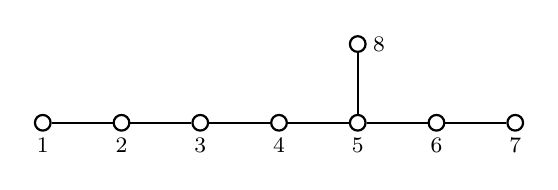
\begin{tikzpicture}[scale=1.0]
  \foreach \i in {1,...,7} { \node[circle,draw,thick,fill=white,inner sep=2pt] (n\i) at (\i,0) {}; \node[below=2pt] at (\i,0) {\footnotesize $\i$}; }
  \node[circle,draw,thick,fill=white,inner sep=2pt] (n8) at (5,1) {};
  \node[right=2pt] at (5,1) {\footnotesize $8$};
  \foreach \i/\j in {1/2,2/3,3/4,4/5,5/6,6/7} \draw[thick] (n\i) -- (n\j);
  \draw[thick] (n5) -- (n8);
\end{tikzpicture}
\zucap{$E_8$ のディンキン図形。頂点 $5$ から長さ $4,2,1$ の腕（$\{1,2,3,4\}$, $\{6,7\}$, $\{8\}$）が出ている。}
\end{center}
(1) 木の形の図形で、端点 $v$ とその隣 $w$ について $\det C=2\det C_{\setminus v}-\det C_{\setminus\{v,w\}}$ を示せ（$C_{\setminus v}$ は $v$ の行と列を除いたもの）。\\
(2) $\det A_n=n+1$, $\det D_n=4$（$n\ge3$；$D_3=A_3$）を認めて、$\det E_6=3$, $\det E_7=2$, $\det E_8=1$ を示せ。\\
(3) $E_8$ 形式は正定値・偶・ユニモジュラーであることを示し、符号数を答えよ。\\
(4) $E_8$ 形式を交叉形式とする滑らかな閉4次元多様体は存在しないことを、ロホリンの定理から説明せよ（単連結な場合、偶な交叉形式ならスピンであることを用いてよい）。
\end{problem}

\begin{solution}
(1) $v$ の行で余因子展開する。$v$ の行の非零成分は $C_{vv}=2$ と $C_{vw}=-1$ だけ。$C_{vv}$ の余因子は $\det C_{\setminus v}$。$C_{vw}$ の余因子は、$v$ 行と $w$ 列を除いた小行列で、その中で $v$ 列の非零成分は $C_{wv}=-1$（$w$ 行）だけなので、さらに $v$ 列で展開して $\pm C_{wv}\det C_{\setminus\{v,w\}}$ になる。符号を整理すると、一般に（対称行列で $v$ が葉のとき）
\[
\det C=C_{vv}\det C_{\setminus v}-C_{vw}C_{wv}\det C_{\setminus\{v,w\}}=2\det C_{\setminus v}-\det C_{\setminus\{v,w\}} .
\]
\begin{note}
符号の確認：$\det C=\sum_\pi\operatorname{sgn}\pi\prod_iC_{i\pi(i)}$ で、$\pi(v)=v$ の項の和が $2\det C_{\setminus v}$。$\pi(v)=w$ の項では、$v$ 列の非零成分は $v$ 行と $w$ 行だけで $v$ 行はすでに使ったので $\pi(w)=v$。よって $\pi$ は互換 $(v\,w)$ と $C_{\setminus\{v,w\}}$ 上の置換の積で、符号は $-1$ 倍、寄与は $-C_{vw}C_{wv}\det C_{\setminus\{v,w\}}=-\det C_{\setminus\{v,w\}}$。
\end{note}

(2) $E_8$ で長い腕の端 $v=1$, $w=2$ をとる。$E_8\setminus\{1\}$ は腕の長さ $3,2,1$ で $E_7$、$E_8\setminus\{1,2\}$ は腕 $2,2,1$ で $E_6$。同様に $E_6\setminus\{3\}$ は腕 $1,2,1$ で $D_5$、$E_6\setminus\{3,4\}$ は頂点 $5,6,7,8$ の鎖で $A_4$。$E_7\setminus\{2\}=E_6$、$E_7\setminus\{2,3\}=D_5$。したがって
\begin{align*}
\det E_6&=2\det D_5-\det A_4=2\cdot4-5=3,\\
\det E_7&=2\det E_6-\det D_5=2\cdot3-4=2,\\
\det E_8&=2\det E_7-\det E_6=2\cdot2-3=1 .
\end{align*}
（$\det D_5=4$ も同じ漸化式 $\det D_5=2\det D_4-\det D_3=8-4$ で確かめられる。）

(3) 単純リー環の単純ルート $\alpha_i$（長さの2乗 $2$ に規格化）の内積行列がカルタン行列 $C_{ij}=\alpha_i\cdot\alpha_j$ であり（単純レース型）、線形独立なベクトルのグラム行列なので正定値。$\det=1$ でユニモジュラー。$x\in\Z^8$ に対し
\[
x^{\mathsf T}Cx=\sum_i2x_i^2-2\sum_{\langle ij\rangle}x_ix_j\in2\Z
\]
（$\langle ij\rangle$ は辺）なので偶。正定値なので $b_+=8$, $b_-=0$, $\sigma=8$。これは「偶ユニモジュラーなら $\sigma\equiv0\pmod8$」の最小の例である。

(4) $X$ が交叉形式 $E_8$ の滑らかな閉4次元多様体なら、$\sigma=8$。単連結と仮定すると、偶な交叉形式なのでウー公式から $w_2=0$、すなわちスピン。ロホリンの定理は $\sigma\equiv0\pmod{16}$ を要求するが $8\not\equiv0$ で矛盾。（単連結でない場合も、$\pi_1$ の仮定を外した形のドナルドソンの定理「滑らかな閉4次元多様体の定値な交叉形式は対角化可能」により否定される。$E_8$ 形式は偶なので $\operatorname{diag}(1,\dots,1)$ と同型でない。）なお位相多様体としては $E_8$ 多様体が存在し（フリードマン）、「滑らかさ」が本質的である。弦理論では、16次元の偶ユニモジュラー正定値格子 $E_8\oplus E_8$ と $\mathrm{Spin}(32)/\Z_2$ の格子が、ヘテロティック弦の2つのゲージ群を与える（モジュラー不変性が偶ユニモジュラー性を要求する）。
\end{solution}

\begin{problem}[難易度 C]\label{ch06-prob-k3}
K3 曲面 $X$ は単連結なコンパクト複素曲面で、$\chi(X)=24$, $\sigma(X)=-16$、スピン多様体であることを認める。\\
(1) $b_0,\dots,b_4$ と $b_\pm$ を求めよ。\\
(2) セールの分類を用いて、交叉形式が $3H\oplus2(-E_8)$ であることを示せ。行列式と符号数を確かめよ。\\
(3) ロホリンの定理との整合性を確かめよ。また、ヒルツェブルフの符号数定理 $\sigma=\frac13\int p_1$ と $\Ahat$ 種数 $\int\Ahat=-\frac{1}{24}\int p_1$ から、K3 上のディラック作用素の指数を求めよ（第9章で扱う公式を認めてよい）。\\
(4) IIA 型弦理論を K3 にコンパクト化すると、6次元の $U(1)$ ゲージ場の個数は $b_0+b_2+b_4$ で与えられる（RR 場 $C_1$ と $C_3$ を偶数次のサイクルで展開することによる）。この個数を求めよ。
\end{problem}

\begin{solution}
(1) 単連結なので $H_1=0$、$b_1=0$。ポアンカレ双対で $b_3=b_1=0$。連結かつ向き付け可能（複素多様体）なので $b_0=b_4=1$。$\chi=b_0-b_1+b_2-b_3+b_4=2+b_2=24$ より $b_2=22$。$b_++b_-=22$, $b_+-b_-=-16$ を解いて $b_+=3$, $b_-=19$。

(2) 単連結なので $H^2(X;\Z)=\Hom(H_2,\Z)\oplus\Ext(H_1,\Z)$ は自由で階数22。スピンなので交叉形式は偶（ウー公式）。$b_+=3>0$, $b_-=19>0$ なので不定値。セールの分類から $Q\cong aH\oplus bE_8$ で、階数 $2a+8\lvert b\rvert=22$、符号数 $0\cdot a+8b=-16$。よって $b=-2$、$a=3$ で $Q\cong3H\oplus2(-E_8)$。
確認：$\det(3H\oplus2(-E_8))=(\det H)^3(\det(-E_8))^2=(-1)^3\cdot((-1)^8\cdot1)^2=-1$ でユニモジュラー。符号数は $H$ が $0$、$-E_8$ が $-8$ ずつで $-16$。

(3) $\sigma=-16\equiv0\pmod{16}$ でロホリンの定理と整合する。$\int p_1=3\sigma=-48$、$\int\Ahat=-\frac{-48}{24}=2$。指数定理（第9章）より、K3 上のディラック作用素の指数は $\ind\slashed D=\int\Ahat=2$。（実際 K3 はハイパーケーラーで、正カイラリティの平行なスピノルが2つある。）ロホリンの定理は、4次元スピン多様体では $\ind\slashed D=-\sigma/8$ が偶数（四元数構造によりゼロモードが対で現れる）であることから従う：$-\sigma/8\in2\Z\iff\sigma\in16\Z$。K3 は $-\sigma/8=2$ でこの最小例である。

(4) $b_0+b_2+b_4=1+22+1=24$ 個。$C_1$ から1個（$b_0$）、$C_3$ を22個の調和2形式で展開して22個（$b_2$）、$C_3$ の6次元での双対（$b_4$）から1個。電荷格子は偶数次のコホモロジー $H^0\oplus H^2\oplus H^4$ に（交叉形式で）内積を入れた格子 $(3H\oplus2(-E_8))\oplus H\cong4H\oplus2(-E_8)$ で、符号数 $(4,20)$ の偶ユニモジュラー格子 $\Gamma^{4,20}$ となり、$T^4$ 上のヘテロティック弦の格子と一致する（IIA/K3 とヘテロティック/$T^4$ の双対性の証拠の1つ；第10章で扱う）。
\end{solution}

\begin{problem}[難易度 C]\label{ch06-prob-theta}
$X$ を向き付けられた4次元閉多様体（ユークリッド時空）とし、$U(1)$ ゲージ理論に $\theta$ 項 $S_\theta=\frac{\theta}{8\pi^2}\int_XF\wedge F$ を加える。経路積分の重みは $e^{iS_\theta}$ を含み、すべての $U(1)$ 束（$c=[F/2\pi]\in H^2(X;\Z)$）について和をとるとする。\\
(1) $S_\theta=\frac\theta2Q_X(c,c)$ を示せ。\\
(2) $X$ がスピン多様体（交叉形式が偶）なら $\theta\sim\theta+2\pi$ であることを示せ。\\
(3) $X=\CP^2$ では $S_\theta=\frac\theta2n^2$（$n\in\Z$）となること、$\theta\to\theta+2\pi$ で重みが $(-1)^n$ 倍され、周期が $4\pi$ になることを示せ。\\
(4) ウー公式を用いると、一般の $X$ で $\theta\to\theta+2\pi$ による重みの変化は $(-1)^{\langle\bar c\smile w_2,[X]\rangle}$ と書けることを示し、物理的な意味を述べよ。
\end{problem}

\begin{solution}
(1) 物理との対応「$U(1)$ 流束とインスタントン数」より、$F/2\pi$ はド・ラーム類として $c$ の実像を代表し、ド・ラームの同型は積を保つので
\[
\frac{1}{4\pi^2}\int_XF\wedge F=\int_X\frac F{2\pi}\wedge\frac F{2\pi}=\langle c\smile c,[X]\rangle=Q_X(c,c).
\]
よって $S_\theta=\frac{\theta}{8\pi^2}\int F\wedge F=\frac\theta2Q_X(c,c)$。$U(1)$ のインスタントン数は $k=\frac12Q_X(c,c)$。

(2) 偶なら $Q_X(c,c)=2m$（$m\in\Z$）、$S_\theta=\theta m$。$\theta\to\theta+2\pi$ で $e^{iS_\theta}\to e^{iS_\theta}e^{2\pi im}=e^{iS_\theta}$。すべての束の重みが不変なので理論は同じであり、$\theta$ の周期は $2\pi$。$S^2\times S^2$（$Q(c,c)=2ab$）、$T^4$（$2\Pf(n)$）、K3 がこの場合である。

(3) $H^2(\CP^2;\Z)=\Z x$, $Q(x,x)=1$。$c=nx$（$n=\frac1{2\pi}\int_{\CP^1}F$）なら $Q(c,c)=n^2$、$S_\theta=\frac\theta2n^2$。$\theta\to\theta+2\pi$ で重みは $e^{i\pi n^2}=(-1)^{n^2}=(-1)^n$ 倍され、$n$ 奇数のセクターの符号が反転するので理論は変わる。$\theta\to\theta+4\pi$ では $e^{2\pi in^2}=1$ で不変。よって周期は $4\pi$。$k=n^2/2$ は半整数をとる。

(4) ウー公式 $Q(c,c)\equiv\langle\bar c\smile w_2,[X]\rangle\pmod2$ より、$\theta\to\theta+2\pi$ で重みは $e^{i\pi Q(c,c)}=(-1)^{\langle\bar c\smile w_2,[X]\rangle}$ 倍される。スピン多様体（$w_2=0$）では常に $1$ で (2) と一致し、$\CP^2$ では $w_2=\bar x$（$c_1(T\CP^2)=3x$ の mod 2 還元）なので $(-1)^n$ で (3) と一致する。
物理的意味：$\theta\to\theta+2\pi$ のずれは、ゲージ場と時空の幾何（$w_2$）の混合した位相項 $\pi\int\bar c\smile w_2$ にすぎない。この項は局所的な自由度をもたないので、「$\theta$ の周期は $2\pi$ だが、$\theta\to\theta+2\pi$ で重力との混合位相項がずれる」と言い換えることもできる。また、フェルミオンを含む理論で非スピン多様体を扱うには spin$^c$ 構造を用い、そのとき $F/2\pi$ の量子化条件自体が $w_2$ だけずれる（第9章で扱う）。いずれにせよ、$\theta$ の周期性は時空のコホモロジー環（交叉形式の偶奇）に依存する。
\end{solution}

\subsection{絡み数とチャーン・サイモンズ理論}

\begin{problem}[難易度 D]\label{ch06-prob-cs}
(1) $\R^3$ 内の交わらない閉曲線 $C_1,C_2$ について、ガウスの積分 $\mathrm{Lk}(C_1,C_2)$（動機の節）は、$C_1$ を流れる単位電流が作るビオ・サバールの磁場
\[
\bm B_1(\bm x)=\frac1{4\pi}\oint_{C_1}\frac{d\bm x_1\times(\bm x-\bm x_1)}{\lvert\bm x-\bm x_1\rvert^3}
\]
の周回積分 $\oint_{C_2}\bm B_1\cdot d\bm x_2$ に等しいことを示せ。アンペールの法則（$\nabla\times\bm B_1$ は $C_1$ に沿った単位電流）を用いて、これが $C_1\cdot S_2$（$S_2$ は $C_2$ が張る曲面）に等しく整数であることを示せ。\\
(2) $C_1(s)=(\cos s,\sin s,0)$, $C_2(t)=(1+\cos t,0,-\sin t)$（$s,t\in[0,2\pi]$）は交わらないことを確かめ、$\mathrm{Lk}(C_1,C_2)=+1$ を示せ（ホップ絡み目）。\\
(3) アーベリアン・チャーン・サイモンズ理論 $S=\frac k{4\pi}\int_{\R^3}A\wedge dA+\sum_jq_j\oint_{C_j}A$ を考える（重み $e^{iS}$、$A$ は $U(1)$ ゲージ場、$q_j\in\Z$）。ベクトル表示で $A\wedge dA=\bm A\cdot(\nabla\times\bm A)\,d^3x$、源の項を $\int\bm A\cdot\bm J\,d^3x$ と書く。運動方程式 $\frac k{2\pi}\nabla\times\bm A=-\bm J$ を導き（\textbf{流束の付着}）、作用の停留値が $S_*=\frac12\int\bm A_*\cdot\bm J\,d^3x$ であることを示せ。ガウス積分では $\langle\prod_jW_{q_j}(C_j)\rangle\propto e^{iS_*}$ であることを認めて、
\[
\bigl\langle W_{q_1}(C_1)W_{q_2}(C_2)\bigr\rangle\propto\exp\Bigl(-\frac{2\pi i}{k}q_1q_2\,\mathrm{Lk}(C_1,C_2)\Bigr)
\]
を示せ（比例係数は各ループ単独の寄与で、$C_1,C_2$ の相対位置によらない）。これがエニオンの組みひも位相にあたることを説明せよ。
\end{problem}

\begin{solution}
(1) $\oint_{C_2}\bm B_1\cdot d\bm x_2=\frac1{4\pi}\oint\oint\frac{(d\bm x_1\times(\bm x_2-\bm x_1))\cdot d\bm x_2}{\lvert\bm x_2-\bm x_1\rvert^3}$。スカラー三重積の巡回性より
\[
(d\bm x_1\times(\bm x_2-\bm x_1))\cdot d\bm x_2=(\bm x_2-\bm x_1)\cdot(d\bm x_2\times d\bm x_1)=(\bm x_1-\bm x_2)\cdot(d\bm x_1\times d\bm x_2),
\]
これはガウスの積分の被積分関数そのもの。よって $\mathrm{Lk}(C_1,C_2)=\oint_{C_2}\bm B_1\cdot d\bm x_2$。
$C_2$ が張る向き付き曲面 $S_2$ をとり（$C_1$ と横断的に交わるとする）、ストークスの定理を使うと $\oint_{C_2}\bm B_1\cdot d\bm x=\int_{S_2}(\nabla\times\bm B_1)\cdot d\bm S$。$\nabla\times\bm B_1=\bm J_1$ は $C_1$ に集中した単位電流 $\bm J_1(\bm x)=\oint_{C_1}d\bm x_1\,\delta^3(\bm x-\bm x_1)$ なので、右辺は $C_1$ が $S_2$ を貫く各点で $\pm1$（$C_1$ の向きが $S_2$ の法線と同じなら $+1$）の和、すなわち $C_1\cdot S_2\in\Z$。
\begin{note}
$\bm B_1$ は $C_1$ 上で特異だが、$C_1\cap C_2=\emptyset$ なので $C_2$ の近くでは滑らかであり、$\bm B_1$ のビオ・サバール表示から $\nabla\cdot\bm B_1=0$、$\nabla\times\bm B_1=\bm J_1$（超関数の意味）が従う。$S_2$ を別の曲面 $S_2'$ に取り替えると、差 $S_2-S_2'$ は閉曲面で、それを $C_1$ が貫く符号付き回数は $0$（閉曲線は閉曲面の内部に入ったら出る）なので、$C_1\cdot S_2$ は $S_2$ によらない。
\end{note}

(2) $C_2$ 上の点で $C_1$ に乗りうるのは $z=-\sin t=0$ の点 $(2,0,0)$, $(0,0,0)$ だけで、どちらも $\lvert\bm x\rvert\neq1$ なので交わらない。$C_2$ は $xz$ 平面内の中心 $(1,0,0)$、半径1の円で、$S_2$ をその円板とする。$t=0$ で $C_2=(2,0,0)$、接ベクトル $(0,0,-1)$。中心から外向きの $(1,0,0)$ と接ベクトルの外積 $(1,0,0)\times(0,0,-1)=(0,1,0)$ が、境界の向きと右ねじの関係にある法線である（円の向きを $\bm r\times\dot{\bm r}$ で判定）。$C_1$ は円板と $(1,0,0)$（$s=0$）でただ1回交わり、そこでの接ベクトルは $(0,1,0)$ で法線と同じ向き。よって $\mathrm{Lk}=C_1\cdot S_2=+1$。（$C_1$ は $z=0$ 平面内にあり、$xz$ 平面とは $(\pm1,0,0)$ で交わるが、$(-1,0,0)$ は円板の外。）

(3) 変分：$\delta\int\bm A\cdot(\nabla\times\bm A)=\int\bigl(\delta\bm A\cdot\nabla\times\bm A+\bm A\cdot\nabla\times\delta\bm A\bigr)=2\int\delta\bm A\cdot(\nabla\times\bm A)$（部分積分で表面項を落とす）。よって
\[
\delta S=\int\delta\bm A\cdot\Bigl(\frac k{2\pi}\nabla\times\bm A+\bm J\Bigr)d^3x=0\ \Longrightarrow\ \frac k{2\pi}\nabla\times\bm A_*=-\bm J .
\]
第3成分を時間とみると $(\nabla\times\bm A)_3$ は磁場なので、静止した電荷 $q$ の粒子の位置に磁束 $-2\pi q/k$ が付着する（粒子が電荷と磁束を同時にもつ）。停留値は
\[
S_*=\frac k{4\pi}\int\bm A_*\cdot\Bigl(-\frac{2\pi}k\bm J\Bigr)+\int\bm A_*\cdot\bm J=\frac12\int\bm A_*\cdot\bm J .
\]
$\bm J=\sum_jq_j\bm J_j$ とし、$\nabla\times\bm B_j=\bm J_j$ をみたすビオ・サバール場 $\bm B_j$ を用いると $\bm A_*=-\frac{2\pi}k\sum_jq_j\bm B_j$（ゲージ変換を除く；$\bm J$ が保存するので源の項はゲージ不変）。よって
\[
S_*=-\frac\pi k\sum_{i,j}q_iq_j\int\bm B_i\cdot\bm J_j\,d^3x=-\frac\pi k\sum_{i,j}q_iq_j\oint_{C_j}\bm B_i\cdot d\bm x .
\]
$i\neq j$ の項は (1) より $\oint_{C_j}\bm B_i\cdot d\bm x=\mathrm{Lk}(C_i,C_j)$ で、$(i,j)=(1,2),(2,1)$ の2項から
\[
S_*=-\frac{2\pi}kq_1q_2\,\mathrm{Lk}(C_1,C_2)+(\text{$i=j$ の項}).
\]
$i=j$ の項（自己絡み）は各ループ単独で決まり、定義には枠付け（フレーミング）が必要だが、$C_1,C_2$ の相対位置によらない。よって $\langle W_{q_1}W_{q_2}\rangle\propto\exp\bigl(-\frac{2\pi i}kq_1q_2\mathrm{Lk}\bigr)$。

エニオン：$2+1$ 次元時空で、電荷 $q_2$ の粒子が電荷 $q_1$ の粒子のまわりを一周する過程の世界線は、（対生成・対消滅で閉じると）$\mathrm{Lk}=\pm1$ の絡み目になる。その振幅は絡んでいない場合と比べて位相 $e^{\mp2\pi iq_1q_2/k}$ だけ異なり、これが組みひも（ブレイディング）の位相である。$q_1q_2/k\notin\Z$ なら位相は自明でなく、粒子はボソンでもフェルミオンでもない統計（エニオン）に従う。この位相は時空の計量によらず、絡み数という位相不変量だけで決まる。分数量子ホール状態（$\nu=1/k$ のラフリン状態）の準粒子の分数統計はこの仕組みによる。
\end{solution}
